% For submission.
\documentclass[sigconf]{acmart}

\graphicspath{{fig/}}

% Already loaded in acmart:
% - microtype
% - fontenc
% - graphicx

\usepackage[utf8]{inputenc}
\usepackage{url}
\usepackage{amsmath,amssymb,bm,mathtools}
\usepackage{bbm}
\usepackage{subfig}
\usepackage{numprint}

% Email.
% \newcommand{\email}[1]{\href{mailto:#1}{\nolinkurl{#1}}}
% Arg{sort, min, max}.
\DeclareMathOperator*{\argsort}{arg\,sort}
\DeclareMathOperator*{\argmax}{arg\,max}
\DeclareMathOperator*{\argmin}{arg\,min}
% Shortcut CO\textsubscript{2}.
\newcommand\COtwo{CO\textsubscript{2}}
% "Given" symbol.
\newcommand\given{\:\vert\:}
% Vectors in bold
\renewcommand{\vec}[1]{\boldsymbol{#1}}
% "Transpose" symbol.
\newcommand{\tr}{^\intercal}

% Legislatures.
\renewcommand{\th}{\textsuperscript{th} }
\newcommand{\rd}{\textsuperscript{rd} }
\newcommand{\ep}[1]{EP#1}
% \newcommand{\ep8}{EP8}


\newcolumntype{L}[1]{>{\raggedright\let\newline\\\arraybackslash\hspace{0pt}}m{#1}}
\newcolumntype{C}[1]{>{\centering\let\newline\\\arraybackslash\hspace{0pt}}m{#1}}
\newcolumntype{R}[1]{>{\raggedleft\let\newline\\\arraybackslash\hspace{0pt}}m{#1}}

% Removes double spacing after end of sentence.
% See: http://practicaltypography.com/one-space-between-sentences.html.
\frenchspacing

%% Rights management information.  This information is sent to you
%% when you complete the rights form.  These commands have SAMPLE
%% values in them; it is your responsibility as an author to replace
%% the commands and values with those provided to you when you
%% complete the rights form.
\setcopyright{iw3c2w3}
\copyrightyear{2020}
\acmYear{2020}
\acmDOI{10.1145/3366423.3380041}

%% These commands are for a PROCEEDINGS abstract or paper.
\acmConference[WWW '20]{Proceedings of The Web Conference 2020}{April 20--24, 2020}{Taipei, Taiwan}
\acmBooktitle{Proceedings of The Web Conference 2020 (WWW '20), April 20--24, 2020, Taipei, Taiwan}
\acmPrice{}
\acmISBN{978-1-4503-7023-3/20/04}
%% Update ISBN for Proceedings or Companion, can be found on completed rightsreview form

\settopmatter{printacmref=true}

\begin{document}

% The "title" command has an optional parameter, allowing the author to define a "short title" to be used in page headers.
\title[The Competitive Dynamics of Legislative Processes]{War of Words: The Competitive Dynamics \texorpdfstring{\\of Legislative Processes}{}}

% The "author" command and its associated commands are used to define the authors and their affiliations.
% Of note is the shared affiliation of the first two authors, and the "authornote" and "authornotemark" commands
% used to denote shared contribution to the research.
\author{Victor Kristof}
\affiliation{%
	% \institution{Ecole polytechnique fédérale de Lausanne}
	\institution{EPFL}
}
% \email{victor.kristof@epfl.ch}

\author{Matthias Grossglauser}
\affiliation{%
	\institution{EPFL}
}
% \email{matthias.grossglauser@epfl.ch}

\author{Patrick Thiran}
\affiliation{%
	\institution{EPFL}
}
% \email{patrick.thiran@epfl.ch}

% By default, the full list of authors will be used in the page headers. Often, this list is too long, and will overlap
% other information printed in the page headers. This command allows the author to define a more concise list
% of authors' names for this purpose.
% \renewcommand{\shortauthors}{V. Kristof et al.}

\begin{abstract}
	% Max 250 wrods, c.f. https://wordcounter.net/.
As the number of contributors to online peer-production systems grows, it becomes increasingly important to predict whether the edits that users make will eventually be beneficial to the project.
Existing solutions either rely on a user reputation system or consist of a highly specialized predictor that is tailored to a specific peer-production system.
In this work, we explore a different point in the solution space that goes beyond user reputation but does not involve any content-based feature of the edits.
We view each edit as a game between the editor and the component of the project.
We posit that the probability that an edit is accepted is a function of the editor's skill, of the difficulty of editing the component and of a user-component interaction term.
Our model is broadly applicable, as it only requires observing data about \emph{who} makes an edit, \emph{what} the edit affects and whether the edit survives or not.
We apply our model on Wikipedia and the Linux kernel, two examples of large-scale peer-production systems, and we seek to understand whether it can effectively predict edit survival:
in both cases, we provide a positive answer.
Our approach significantly outperforms those based solely on user reputation and bridges the gap with specialized predictors that use content-based features.
It is simple to implement, computationally inexpensive, and in addition it enables us to discover interesting structure in the data.

%We apply it to Wikipedia and the Linux kernel, two examples of large-scale collaborative projects.
%In both cases, the model enables us (a) to discover interesting structure in the data and (b) to effectively predict whether edits will survive.

\end{abstract}

% The code below is generated by the tool at http://dl.acm.org/ccs.cfm.
% Please copy and paste the code instead of the example below.
% TODO: SHOULD BE FILLED LATER
% \begin{CCSXML}
%   <ccs2012>
%   <concept>
%   <concept_id>10002951.10003227.10003351</concept_id>
%   <concept_desc>Information systems~Data mining</concept_desc>
%   <concept_significance>300</concept_significance>
%   </concept>
%   <concept>
%   <concept_id>10002951.10003260.10003277</concept_id>
%   <concept_desc>Information systems~Web mining</concept_desc>
%   <concept_significance>300</concept_significance>
%   </concept>
%   <concept>
%   <concept_id>10010147.10010257</concept_id>
%   <concept_desc>Computing methodologies~Machine learning</concept_desc>
%   <concept_significance>300</concept_significance>
%   </concept>
%   </ccs2012>
% \end{CCSXML}

% \ccsdesc[300]{Information systems~Data mining}
% \ccsdesc[300]{Information systems~Web mining}
% \ccsdesc[300]{Computing methodologies~Machine learning}

% Keywords. The author(s) should pick words that accurately describe the work being
% presented. Separate the keywords with commas.
% \keywords{\textcolor{red}{discrete choice models, computational social science, human behaviour modelling, dataset, text mining, web mining}}

\maketitle

%! TEX root = ../thesis.tex
\section{Introduction}
\label{kks:sec:intro}

% General context & problem setting
In many competitive sports and games (such as tennis, basketball, chess and electronic sports), the most useful definition of a competitor's skill is the propensity of that competitor to win against an opponent.
It is often difficult to measure this skill \emph{explicitly}:
take basketball for example, a team's skill depends on the abilities of its players in terms of shooting accuracy, physical fitness, mental preparation, but also on the team's cohesion and coordination, on its strategy, on the enthusiasm of its fans, and a number of other intangible factors.
However, it is easy to observe this skill \emph{implicitly} through the outcomes of matches.

% Static models of pairwise comparisons.
In this setting, probabilistic models of pairwise-comparison outcomes provide an elegant and practical approach to quantifying skill and to predicting future match outcomes given past data.
These models, pioneered by~\citet{zermelo1928berechnung} in the context of chess (and by~\citet{thurstone1927law} in the context of psychophysics), have been studied for almost a century.
They posit that each competitor $i$ (i.e., a team or player) is characterized by a latent score $s_i \in \mathbf{R}$ and that the outcome probabilities of a match between $i$ and $j$ are a function of the difference $s_i - s_j$ between their scores.
By estimating the scores $\{ s_i \}$ from data, we obtain an interpretable proxy for skill that is predictive of future match outcomes.
If a competitor's skill is expected to remain stable over time, these models are very effective.
But what if it varies over time?

% Dynamic models.
A number of methods have been proposed to adapt comparison models to the case where scores change over time.
Perhaps the best known such method is the Elo rating system~\citep{elo1978rating}, used by the World Chess Federation for their official rankings.
In this case, the time dynamics are captured essentially as a by-product of the learning rule (c.f. Section~\ref{kks:sec:relwork}).
Other approaches attempt to model these dynamics explicitly~\citep[e.g.,][]{fahrmeir1994dynamic, glickman1999parameter, dangauthier2007trueskill, coulom2008whole}.
These methods greatly improve upon the static case when considering historical data, but they all assume the simplest model of time dynamics (that is, Brownian motion).
Hence, they fail to capture more nuanced patterns such as variations at different timescales, linear trends, regression to the mean, discontinuities, and more.

% KickScore: value proposition.
In this work, we propose a new model of pairwise-comparison outcomes with expressive time-dynamics: it generalizes and extends previous approaches.
We achieve this by treating the score of an opponent $i$ as a time-varying Gaussian process $s_i(t)$ that can be endowed with flexible priors~\citep{rasmussen2006gaussian}.
We also present an algorithm that, in spite of this increased flexibility, performs approximate Bayesian inference over the score processes in linear time in the number of observations so that our approach scales seamlessly to datasets with millions of observations.
This inference algorithm addresses several shortcomings of previous methods: it can be parallelized effortlessly and accommodates different variational objectives.
The highlights of our method are as follows.

\begin{description}
	\item[Flexible Dynamics]
	      As scores are modeled by continuous-time Gaussian processes, complex (yet interpretable) dynamics can be expressed by composing covariance functions.

	\item[Generality]
	      The score of an opponent for a given match is expressed as a (sparse) linear combination of features.
	      This enables, e.g., the representation of a home advantage or any other contextual effect.
	      Furthermore, the model encompasses a variety of observation likelihoods beyond win / lose, based, e.g., on the number of points a competitor scores.

	\item[Bayesian Inference]
	      Our inference algorithm returns a posterior \emph{distribution} over score processes.
	      This leads to better predictive performance and enables a principled way to learn the dynamics (and any other model hyperparameters) by optimizing the log-marginal likelihood of the data.

	\item[Ease of Intepretation]
	      By plotting the score processes $\{ s_i(t) \}$ over time, it is easy to visualize the probability of any comparison outcome under the model.
	      As the time dynamics are described through the composition of simple covariance functions, their interpretation is straightforward as well.
\end{description}

% Contributions & organization.
Concretely, our contributions are threefold.
First, we develop a probabilistic model of pairwise-comparison outcomes with flexible time-dynamics (Section~\ref{kks:sec:model}).
The model covers a wide range of use cases, as it enables
\begin{enuminline}
	\item opponents to be represented by a sparse linear combination of features, and
	\item observations to follow various likelihood functions.
\end{enuminline}
In fact, it unifies and extends a large body of prior work.
Second, we derive an efficient algorithm for approximate Bayesian inference (Section~\ref{kks:sec:inference}).
This algorithm adapts to two different variational objectives;
in conjunction with the ``reverse-KL'' objective, it provably converges to the optimal posterior approximation.
It can be parallelized easily, and the most computationally intensive step can be offloaded to optimized off-the-shelf numerical software.
Third, we apply our method on several sports datasets and show that it achieves state-of-the-art predictive performance (Section~\ref{kks:sec:eval}).
Our results highlight that different sports are best modeled with different time-dynamics.
We also demonstrate how domain-specific and contextual information can improve performance even further;
in particular, we show that our model outperforms competing ones even when there are strong intransitivities in the data.

% Visualization & impact.
In addition to prediction tasks, our model can also be used to generate compelling visualizations of the temporal evolution of skills.
All in all, we believe that our method will be useful to data-mining practitioners interested in understanding comparison time-series and in building predictive systems for games and sports.
%Objects represent players or teams.
%Each datum represents a match with two opponents, in which we observe a winner (e.g., in tennis) or possibly a tie (e.g., in chess) or points (e.g., goals in football).
%The objective is to estimate the score of players or teams over time, in such a way that score differences predict match outcomes accurately.

\paragraph{A Note on Extensions}
In this paper, we focus on \emph{pairwise} comparisons for conciseness.
However, the model and inference algorithm could be extended to multiway comparisons or partial rankings over small sets of opponents without any major conceptual change, similarly to~\citet{herbrich2006trueskill}.
Furthermore, and even though we develop our model in the context of sports, it is relevant to all applications of ranking from comparisons, e.g., to those where comparison outcomes reflect human preferences or opinions~\citep{thurstone1927law, mcfadden1973conditional, salganik2015wiki}.

%! TEX root = ../thesis.tex
\section{The European Legislative Process}
\label{sec:background}

\begin{figure}
	\newcommand{\imgscale}{0.35}
	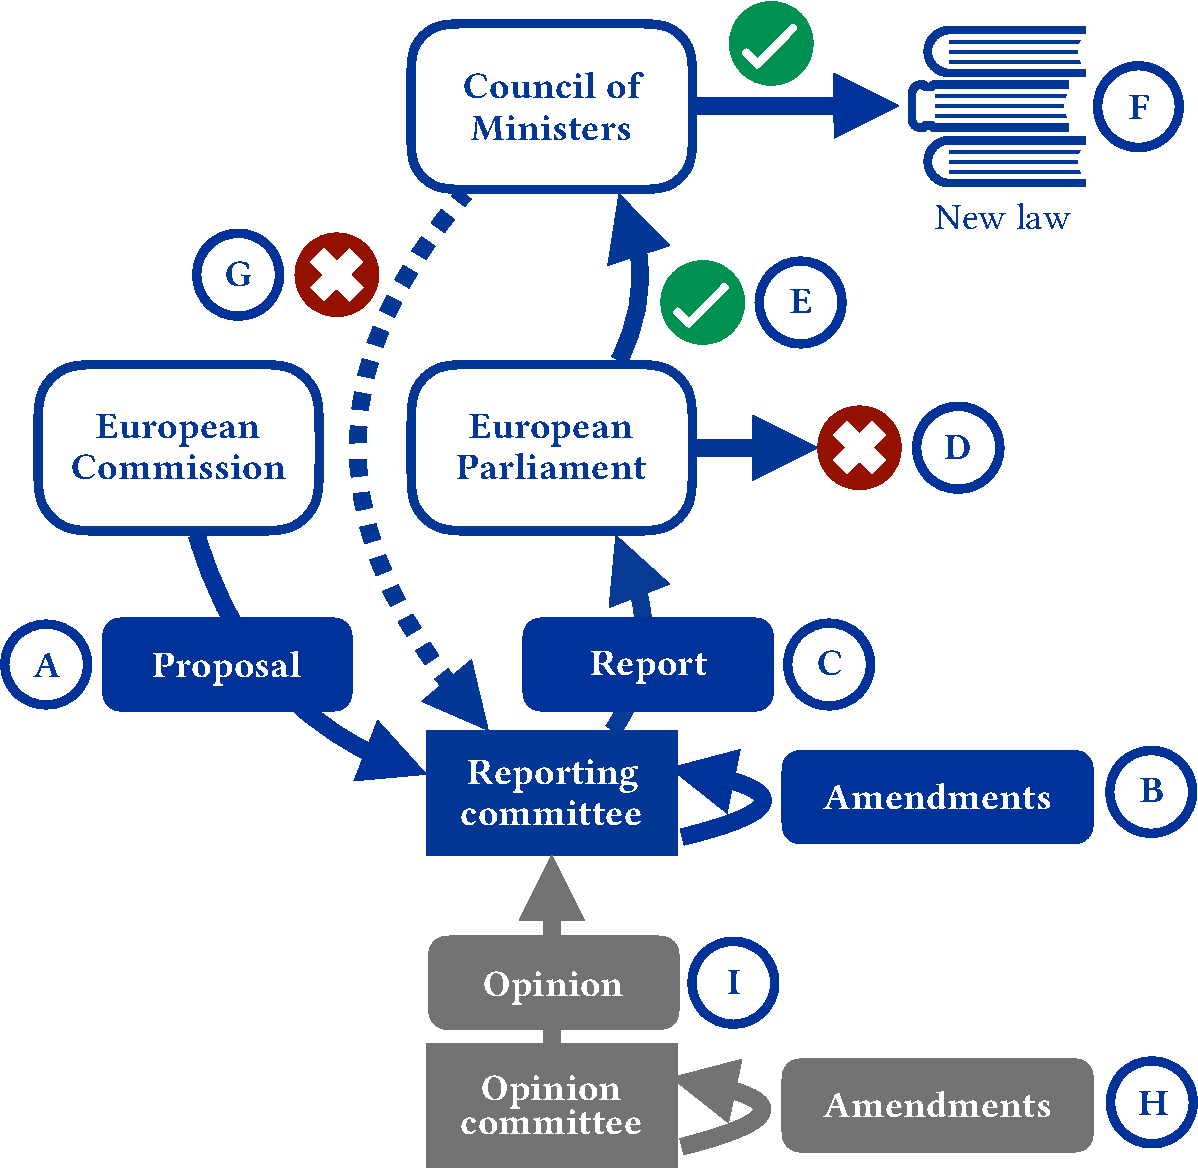
\includegraphics[scale=\imgscale]{lmp-ols}
	\caption{
		Sketch of the \textit{ordinary legislative procedure}.
		(A) The Commission submits a legislative proposal to one of the Parliament committees.
		(B) The proposal is amended and (C) submitted to vote to the whole Parliament.
		(D) If it is rejected, the proposal is abandoned.
		(E) If it is accepted, it is transferred to the Council.
		(F) If the Council accepts the amended proposal, a new law is adopted.
		(G) If the Council amends it, it is sent back to the committee.
		(H) Other committees can optionally make amendments and (I) suggest them to the reporting committee.
	}
	\label{fig:ols}

\end{figure}

\subsection{Representative Democracies}

In representative democracies, citizens elect politicians to represent them in the various branches of the government.
The executive branch is in charge of executing and enforcing the laws.
Representatives of the executive branch can also propose new laws, but, to avoid a concentration of power, they cannot pass new legislation without the approval of the legislative branch.
The legislative branch, typically a parliament, represents both the people and the sub-governmental entities (such as states and municipalities).
Parliamentarians  can propose new legislation or amend propositions made by the executive branch.
Finally, the judicial branch balances the power of the executive branch and the legislative branch through its ability to decide whether the laws are constitutional.

Here, we focus on the European Union (EU).
The EU is a political and economic union of 28 countries called member states.
This union enables them to share their markets, to ease mobility across borders, to favor economic development, and to harmonize laws.
The EU covers an estimated population of 513 million, and up to 84\% of member states' national laws emanate from the EU \cite{miller2010much}.
Hence, EU laws have a significant impact on the life of many people.
European institutions make efforts to be transparent.
They make a lot of valuable data available online: parliamentary amendments, meetings by the commissioners with civil society, and a transparency register to monitor interest groups.
%These efforts give access to large datasets of great value.

The EU political system is broadly similar to that of a regular state.
The 751 parliament representatives (MEPs, for Member of the European Parliament) are elected every five years by universal suffrage.
The executive branch is called the \textit{European Commission}.
The legislative branch consists of the \textit{European Parliament} and of the \textit{Council of Ministers}.
The Parliament is divided into 20 committees, comprising sub-sets of MEPs and specialized in some particular policy area (such as fisheries, judiciary affairs, transportation, and trade).
Each MEP is a member of at least one committee.
The myriad of national parties aggregate into a small number of political groups.

\subsection{The Ordinary Legislative Procedure}

We now describe the EU legislative process in some detail, leading up to our modeling assumptions.
Under the Treaty of Lisbon \cite{eu2007lisbon}, which marks the beginning of the 7\th legislature in 2009, the Parliament's powers were increased.
The Parliament became central in the process through which new laws are created.
This process can take the form of various procedures, the main one being the \textit{ordinary legislative procedure} (OLP)~\cite{europarl2018ordinary}.
Through the OLP, the Commission initiates a legislative proposal, and the Parliament must adopt it in order for the proposal to become a law.
Other procedures exist, where the Parliament is not necessarily involved.
Since 2009, the Parliament has dealt with 90\% of all new laws via the OLP.
In this regard, we focus on the dynamics of the legislative process in the Parliament.
A sketch of the OLP is illustrated in Figure~\ref{fig:ols} and described in the next paragraphs.

To create a new law, (A) the Commission drafts a legislative \textit{proposal} and transfers it to the corresponding committee of the Parliament.
For instance, if the proposal introduces regulations on greenhouse-gas emissions, it is transferred to the Environment Committee.
The committee appoints a \textit{rapporteur} to lead the debate.
The role of the committee is to write a \textit{report} in the form of \textit{amendments} to the proposal, i.e., insertions in or deletions of parts of the proposal.
The rapporteur first seeks external expertise to draft a report.
Then, (B) other MEPs on the committee can in turn propose amendments to the proposal.
To constitute the final report to be submitted to the whole Parliament, each amendment by the rapporteur or by other MEPs is therefore voted on within the committee.
Once the committee finds a consensus, (C) they transfer the report to the whole Parliament.

In the plenary session, the Parliament holds a vote on the report.
(D) If rejected, the proposal is abandoned; (E) if accepted, the report, establishing the Parliament's position on the proposal, is transferred to the Council of Ministers.
The report is therefore an important document and the rapporteur has an important role to play.
The ministers (of the different EU countries) can accept the report, (F) in which case, the proposal is adopted with the Parliament's amendments and a new law is created; or they can make amendments, (G) in which case it is transferred back to the parliamentary committee.
At this stage, we say that a law has gone through the first \textit{reading}.

\begin{table*}
	\caption{Descriptive statistics of the \warofwords\ dataset.}
	\label{tab:dataset}
	\begin{tabular}{cccccccc}
		\toprule
		Legislature      & \# amendments     & \# edits          & \# conflicts     & \# MEPs        & \# dossiers     & \# data points    & \% accepted \\
		\midrule

		EP7 (2009--2014) & \numprint{108292} & \numprint{200407} & \numprint{40302} & \numprint{761} & \numprint{1089} & \numprint{126417} & 37.7\%      \\
		EP8 (2014--2019) & \numprint{128885} & \numprint{249086} & \numprint{56298} & \numprint{791} & \numprint{800}  & \numprint{141034} & 25.7\%      \\

		\bottomrule
	\end{tabular}
\end{table*}

Other committees can also independently decide to address an \textit{opinion} to the reporting committee.
For instance, the Transportation Committee might consider that it is also concerned by greenhouse-gas emissions and that it is entitled to give its opinion to the Environment Committee.
An opinion is similar to a report in that it contains amendments to the proposal.
It is created similarly to a report, i.e., (H) the opinion committee appoints a rapporteur to draft an opinion, and other MEPs can propose amendments.
(I) The opinion committee then transfers its opinion to the reporting committee.
An opinion differs from a report in that it is not voted by the whole Parliament.
Amendments to the opinions are, however, valuable to the reporting committee that often takes them into consideration.
We refer to reports and opinions as \textit{dossiers}.

This iterative process can be repeated up to three times (three readings).
The third reading, called conciliation, involves a negotiation between the Parliament and the Council.
During the 8\th legislature for example, 99\% of all laws were adopted after the first reading, i.e., after amendments made by both the Parliament and the Council, and 89\% were adopted directly after amendments by the Parliament, i.e., the Council accepted it without making amendments.

%! TEX root = ../thesis.tex
\section{Dataset}
\label{lmp:sec:data}

\subsection{Amendments \& Edits}

We collected a dataset of \numprint{237177} legislative amendments from the European Parliament website.\footnote{Data and code publicly available on \href{https://github.com/indy-lab/war-of-words}{https://github.com/indy-lab/war-of-words}.}
The dataset spans the 7\th legislature~(referred to as EP7), from 2009 to 2014, and the 8\th legislature~(EP8), from 2014 to 2019.
MEPs come from 28 different countries, and they belong to one of the 8 (EP7) or 9 (EP8) political groups.
An amendment consists of (i) one or several authors, (ii) the original text by the European Commission, and (iii) the amended text by the author(s).
We show an example of two amendments in their raw format in Figure~\ref{lmp:fig:amendment}.
The two amendments are proposed on Article 13 of a proposal about copyrights on the Internet.
Amendment 802 is proposed by three MEPs and consists of three edits:
(a) Inserting ``copyright'' (in green), (b) replacing ``by'' by ``uploaded by users of'' (in yellow), and (c) deleting the end of the title after ``providers'' (in red).
Amendment 803 is proposed by two other MEPs and consists of two edits:
(d) Replacing ``large'' by ``significant'' (in yellow) and (e) inserting ``copyright protected'' (in green).
There are two conflicts in this amendment:
Edit (c) of the first amendment is in conflict with Edit (d), and it is also in conflict with Edit (e).
All these edits are also implicitly in conflict with the original text proposed by the European Commission.
Out of these five edits, only Edit (d) was accepted.
All other edits were rejected, \textit{i.e.}, the status quo was voted and the text proposed by the Commission was maintained.
% We summarize our dataset in Table~\ref{lmp:tab:dataset} and we refer to it as the \warofwords\ dataset.
% In the next paragraphs, we describe the data that we extract from amendments and that we use for the subsequent analysis.
% We extract \textit{edits} and \textit{conflicts}, and we explain the labelization process.
% Technical details about data processing are given in Appendix~\ref{lmp:sec:dataproc}.

\begin{figure}
  \centering
	\newcommand{\imgscale}{\linewidth*3/4}
	{%
		\setlength{\fboxsep}{5.5pt}%
		\setlength{\fboxrule}{0.5pt}%
		\fbox{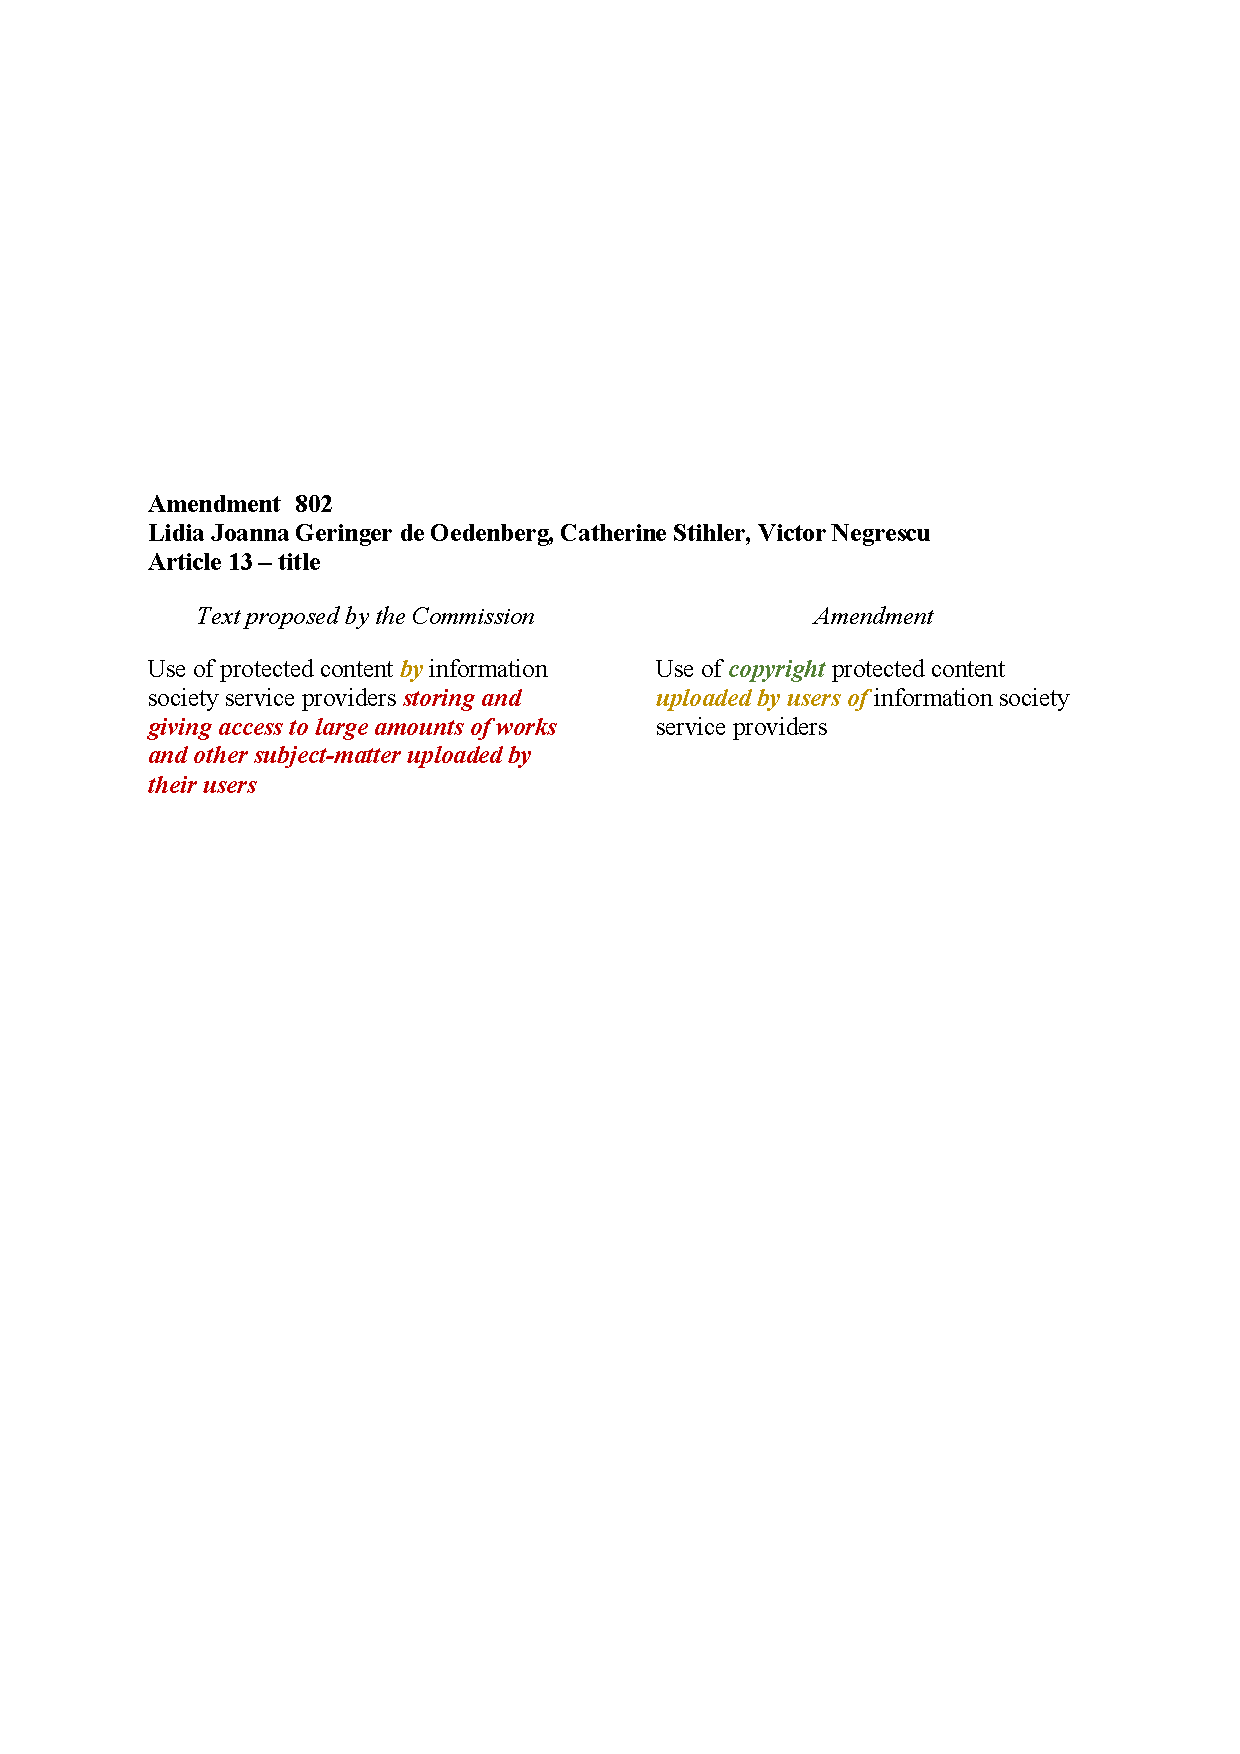
\includegraphics[width=\imgscale]{lmp-amendment-802-colors}}%
	}%
	\vfill
	\vspace{4pt}
	{%
		\setlength{\fboxsep}{5.5pt}%
		\setlength{\fboxrule}{0.5pt}%
		\fbox{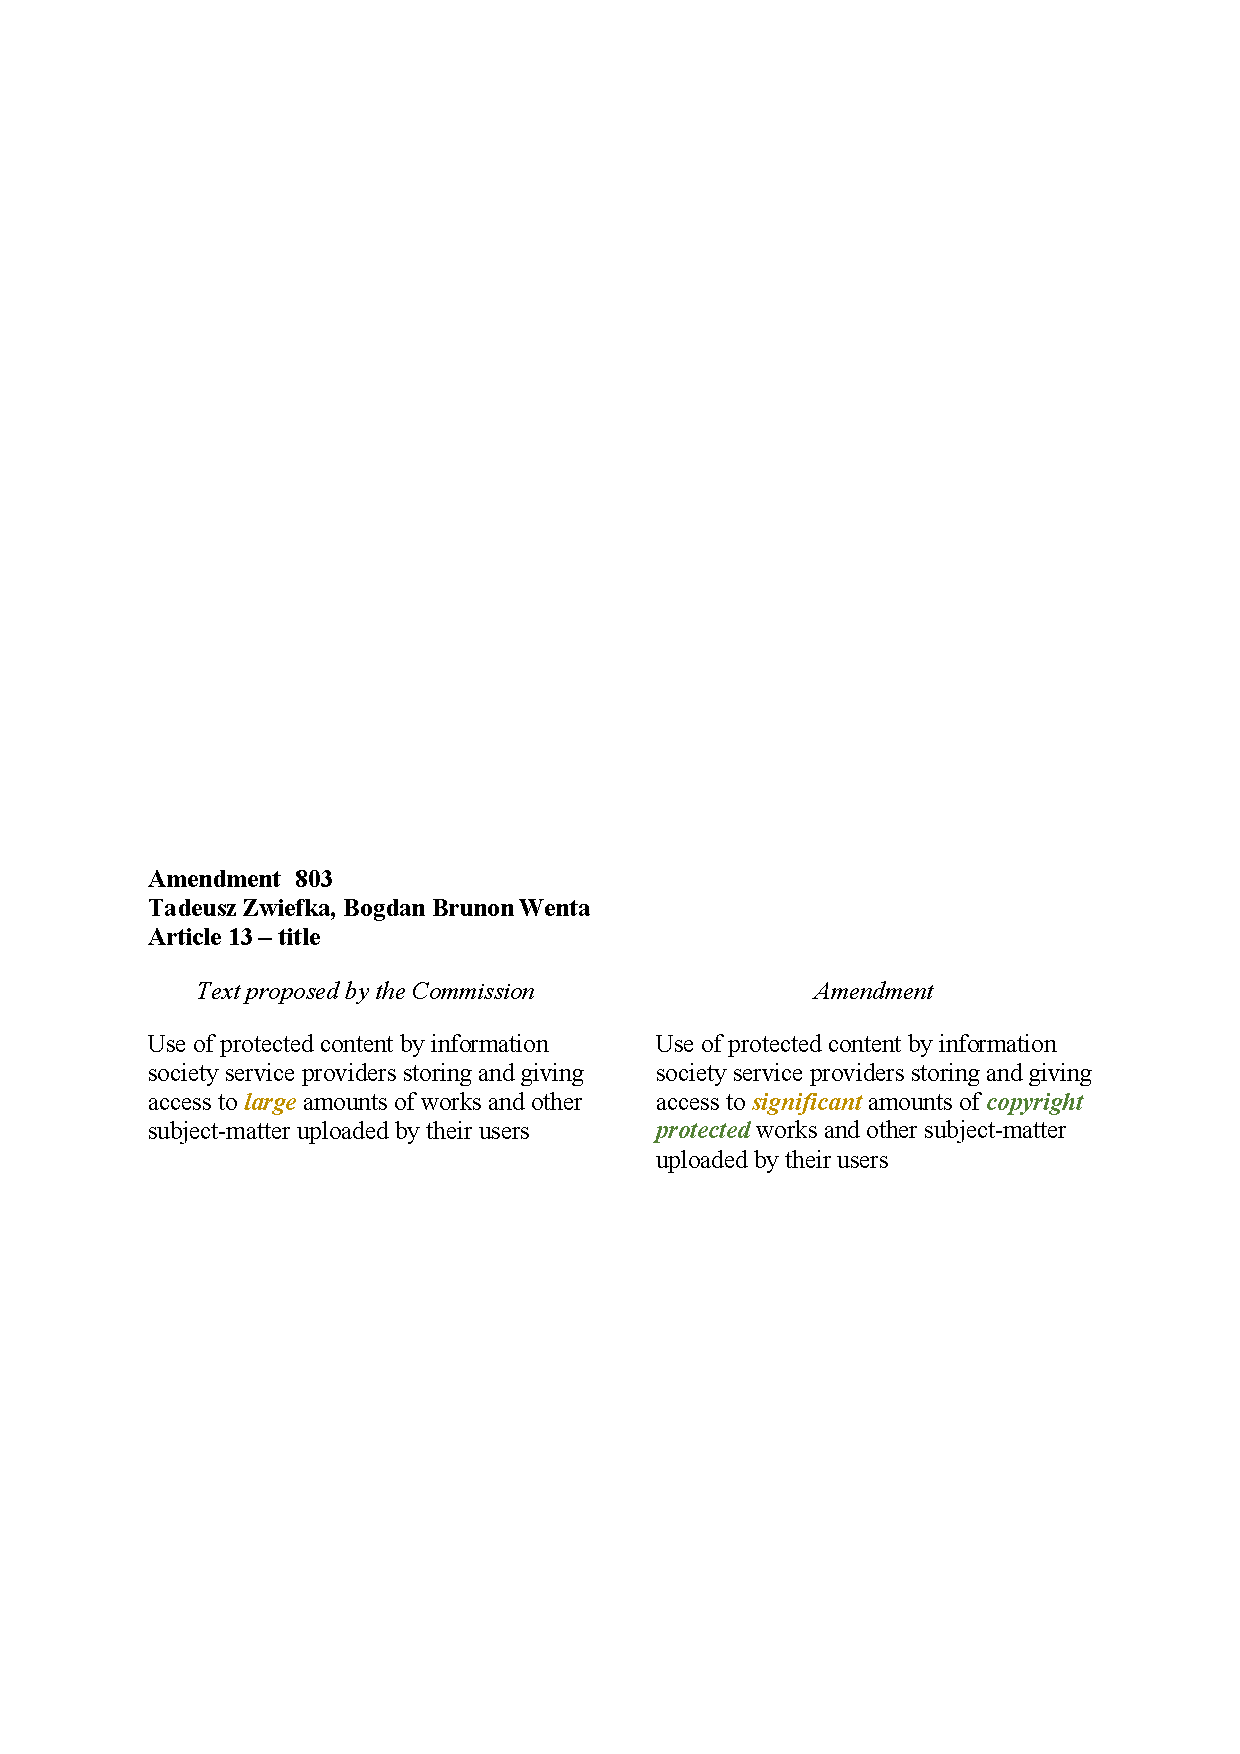
\includegraphics[width=\imgscale]{lmp-amendment-803-colors}}%
	}%
	\caption{
		Example of two conflicting amendments in their raw format on the title of Article 13 of a proposal about copyrights on the Internet.
		(Top) Amendment 802 is proposed by three MEPs and consists of three edits.
		(Bottom) Amendment 803 is proposed by two other MEPs on the same text, and it consists of two edits.
		The last edit of Amendment 802 (deleting the end of the title) conflicts with both edits of Amendment 803.
		Only the first edit of Amendment 803 (replacing ``large'' by ``significant'') was accepted, and all other edits were rejected.
	}
	\label{lmp:fig:amendment}
\end{figure}

\paragraph{Edits}
MEPs propose amendments on a specific article of the legislation, and they can modify several parts within a single amendment.
As a result, we decompose the difference between the original and the amended text into one or several \emph{edits}, as defined below.
An edit is a sequence of words that are inserted or deleted or both.
We extract edits by computing the \emph{diff}, i.e., the difference between the words in two texts, between the original and the amended text of each amendment.
We normalize the texts by removing special characters and by putting the words in lower case.
We keep punctuation because the structure of sentences is important in legal texts.
We merge identical edits proposed by different MEPs, thus considering them as one edit proposed by all authors together.
This is in line with the Rules of Procedure of the Parliament \cite{europarl2018rules}.
We extract \numprint{200407} edits for EP7 and \numprint{249086} edits for EP8.
On average, there are 1.85 and 1.93 edits per amendment for EP7 and EP8, respectively.
There are also more dossiers in EP7 than in EP8, which means that there are proportionally more edits per dossier in EP8.

\paragraph{Conflicts}
There exists an inherent competition between the MEPs in the amending process, as amendments are vehicles of political ideas and interests.
We are therefore interested in the conflicts between edits.
We define a \emph{conflict} as a set of edits that overlap.
Edits overlap because they modify parts of the text at the same position.
We extract \numprint{40302} conflicts for EP7 and \numprint{56298} for EP8.
Adding the conflicts to isolated edits, we obtain a dataset of \numprint{126417} data points for EP7 and \numprint{141034} data points for EP8.

\paragraph{Labels}
The votes on each edit are not publicly available, and we need to infer their outcomes from the raw data.
Reports and opinions contain only the amendments accepted within the committees.
Draft reports, draft opinions, and other documents containing all proposed amendments are published separately.
Therefore, if the edits extracted from the latter documents  appear in the former documents, we label them as \emph{accepted}, i.e., the committee votes to include these edits in their report or opinion.
Otherwise, we label them as \emph{rejected}.
Out of the proposed edits, 37.7\% are accepted for EP7 and 25.7\% for EP8.

\paragraph{Timestamps}
The timeline of the legislative process described in Section~\ref{lmp:sec:background} varies from one dossier to another.
Depending on the dossier, MEPs can propose edits during a window of one to six months, after which all the edits related to that dossier are published together.
As a result, the actual, detailed chronology of the edits is unfortunately hidden, and we do not have access to the precise time the edits are proposed and when they are voted.
Furthermore, there is a delay between the time an edit is proposed and the time it is voted: recent edits might be voted \emph{before} older ones.
The timestamps associated with each edit are, therefore, noisy.

%This departs from reality, because we do not have access to the precise time the edits are proposed and when they are voted.
%We only know when a proposal has reached a reporting committee (respectively, an opinion committee), and when the report (respectively, the opinion) is transferred to the Parliament (respectively, the reporting committee).
%In Section~\ref{lmp:sec:cold-start}, we will explore ways of emulating an amending process that is closer to the actual process.
%As shown in Section~\ref{lmp:sec:results}, these simplistic assumptions enable us, nonetheless, to take advantage of the available data to gain insights into the EU legislative process.


In total, we collect \numprint{449493} edits from \numprint{237177} amendments in the European Parliament during the 7\th and the 8\th legislature periods\footnote{We do not collect data from EP9 (2019 -- 2023), as the amount of published data is too small at this time: The legislature period started in Fall 2019 and the Parliament's activities were slowed down due to the COVID-19 crisis in Spring 2020.} (referred to as EP7 and EP8), between 2009 and 2019 (each period lasts 5 years).
After gathering the edits according to the conflicts, we obtain \numprint{267451} conflicts for both EP7 and EP8, covering 1889 dossiers.
We summarize this dataset in Table~\ref{lmp:tab:dataset}.

\begin{table}
  \centering
	\caption{Descriptive statistics of our extended dataset.}
	\label{lmp:tab:dataset}
	\begin{tabular}{lrr}
		\toprule
    & EP7 (2009--2014) &EP8 (2014--2019) \\
		\midrule
  \# amendments & \numprint{108292} &\numprint{128885}  \\
 \# edits       & \numprint{200407} &\numprint{249086}  \\
 \# conflicts   & \numprint{126417} &\numprint{141034}  \\
 \# MEPs        & \numprint{761}    &\numprint{791}     \\
 \# dossiers    & \numprint{1089}   &\numprint{800}     \\
 \% accepted    & 37.7\%            &25.7\%             \\
 \% inserted    & 37.8\%            &37.9\%             \\
 \% deleted     & 22.0\%            &22.4\%             \\
 \% replaced    & 40.2\%            &39.7\%             \\
		\bottomrule
	\end{tabular}
\end{table}

\subsection{Explicit Features}

% - What we add and how we collected these data.
%   - Give an example of an amendment
%   - Explain what are the explicit (meta) features and the text features.
We extract explicit (meta) features of the MEPs, the edits, and the dossiers, as well as text features.
For each MEP, we collect their nationality (one of 28), their EU political group (one of 8 or 9), and their gender.
A political group clusters national parties that share similar political ideologies.
For each edit, we identify whether it is an insertion, a deletion, or a replacement of some words in the proposal, and we compute its length.
We also collect information about where in the law the edit was proposed: in an article (in the body of the proposal), in a recital (in the preamble of the proposal), in an annex, or in other more specific but less frequent parts of a law.
We determine whether an edit in a reporting committee comes from an opinion committee (in which case it is an ``outsider'').
Finally, we note whether an edit comes with an optional justification.
For each dossier, we identify its type (report or opinion) and the committee that is in charge.
We also note if the proposal is a regulation (legally binding for all member states of the EU), a directive (sets general goals that member states can implement however they want), or a decision (binding to one member state or company only).
We describe these explicit features in Table~\ref{lmp:tab:features}.

\begin{table}
  \centering
	\caption{List of features for MEPs and edits.}
	\label{lmp:tab:features}
	\begin{tabular}{lll}
		\toprule
		Category & Feature            & Type [Values]                     \\
		\midrule
		MEP      & Nationality        & Categorical [28]                  \\
		         & Political group    & Categorical [8 or 9]              \\
		         & Gender             & Categorical [2]                   \\
		% & Age                 & Categorical [8 or 9] \\
		% & Experience          & Categorical [8 or 9] \\
		         & Rapporteur         & Binary                            \\
		Edit     & Edit type          & Categorical [3]                   \\
		         & Log-length (+)     & Numerical [$\mathbf{R}_{\geq 0}$] \\
		         & Log-length (-)     & Numerical [$\mathbf{R}_{\geq 0}$] \\
		         & Article type       & Categorical [7]                   \\
		         & Outsider committee & Binary                            \\
		         & Justification      & Binary                            \\
		Dossier  & Type               & Categorical [2]                   \\
		         & Committee          & Categorical [35]                  \\
		         & Legal act          & Categorical [3]                   \\
		%         & Directorate-General & Binary \\
		%         & Subject matter      & Binary \\
		%         & Length of proposal  & Binary \\
		\bottomrule
	\end{tabular}
\end{table}

\subsection{Text Features}

We further augment the dataset by collecting text features of the edit itself.
It is reasonable to expect that certain words and phrases are predictive of the success of an edit.
We extract the deleted words~$w_-$ from the proposal and the inserted words~$w_+$ from  the amendment.
In Figure~\ref{lmp:fig:amendment}, for example, Edit (b) of Amendment 802 has~$w_- = \textit{``by''}$ and~$w_+ = \textit{``uploaded by users of''}$.
We also consider the context of an edit by extracting the original text of the whole amended article.
For Amendment 802, the context is the portion of text labelled as \textit{``Text proposed by the Commission''}.
Finally, we also extract the title of the law proposal; we will use it as a text feature of the dossier.
For Amendments 802 and 803, the title is \textit{``Copyright in the Digital Single Market''}.
We map all words to lower case, and we replace digits in the title by the letter ``D'', as there are many reference numbers that are unlikely to be useful for our task.

We give some statistics of the distribution of the length of the deleted text~$w_-$, the inserted text~$w_+$, the context, and the title in Table~\ref{lmp:tab:text}.
We report the lower quartile~$Q_1$ and the upper quartile~$Q_3$, as well as the median.
About half of the inserted and deleted texts are short (7 words or less), but the distribution of lengths has a long tail, as shown by the larger values of the upper quartile~$Q_3$.
The context provides large portions of text (the median is at 42 for EP7 and 49 for EP8), which will be useful for making predictions.
In Section~\ref{lmp:sec:models}, we describe how we incorporate the explicit features and the text features into our models.

\begin{table}
  \centering
	\caption{Distribution of text lengths in number of words.}
	\label{lmp:tab:text}
	\begin{tabular}{llrrr}
		\toprule
		Legislature & Type            & $Q_1$ & Median & $Q_3$ \\
		\midrule
		EP7         & Insertion $w_+$ & 2     & 7      & 20    \\
		            & Deletion $w_-$  & 2     & 6      & 26    \\
		            & Context         & 15    & 42     & 79    \\
		            & Title           & 6     & 12     & 19    \\
		EP8         & Insertion $w_+$ & 2     & 6      & 17    \\
		            & Deletion $w_-$  & 2     & 6      & 28    \\
		            & Context         & 20    & 49     & 93    \\
		            & Title           & 6     & 10     & 22    \\
		\bottomrule
	\end{tabular}
\end{table}

%- Describe the text (give some descriptive statistics, some plots, ...).
% - Distribution of edit length
% - How many amendments have justification
% - Most frequent words and bigrams
% - Count identical edits/amendments

%! TEX root = ../thesis.tex
\section{Edit Graph}
\label{lmp:sec:collconf}

We describe the dynamics of the legislative process in terms of the conflicts between edits.
%We take a graph theoretical approach to explain our model in Section~\ref{lmp:sec:models}.
For each dossier, we construct the edit graph $ G = (V_G, E_G) $, such that each node $ v \in V_G $ is an edit and such that there is an undirected edge $ (u, v) \in E_G $ if edits $u$ and $v$ overlap.
A component of size at least~2 in $G$ is therefore a group of overlapping edits. % removed ``connected'' -> it's part of the definition of ``component'', so unnecessary
An isolated node corresponds to an edit that does not overlap with any other edit.

In Figure~\ref{lmp:fig:edit_graph}, we show the edit graphs of three regulations of EP7.
We depict each node with a green dot if the edit is accepted, and with a red cross if the edit is rejected.
The ``transportable pressure equipment'' (left), a very specific legislation, exhibits a graph with 96 nodes, among which 97\% are accepted.
The graph contains only isolated nodes, meaning that no edits overlap: all its components are size 1.
The ``European capitals of culture'' (center), which can affect some cities of member states, exhibits a graph with 58 nodes, among which 48\% are accepted.
The graph contains 16 cliques and the average component size is 1.49.
The GDPR (right), with high stakes for both businesses and consumers, exhibits a graph with 3154 nodes, among which only 9\% are accepted.
The graph contains 1298 cliques, meaning that many edits are conflicting, and has an average component size of 3.44.

\begin{figure}
  \centering
	\newcommand{\imgscale}{0.88}
	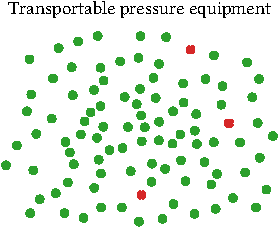
\includegraphics[scale=\imgscale]{lmp-edit-graph-tpe}\hfill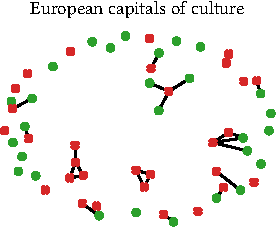
\includegraphics[scale=\imgscale]{lmp-edit-graph-ecc}\hfill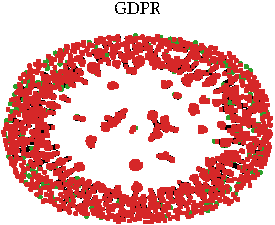
\includegraphics[scale=\imgscale]{lmp-edit-graph-gdpr}
	\caption{
		(Left) The ``transportable pressure equipment'' edit graph contains 96 edits (97\% accepted) and no conflicts.
		(Center) The ``European capitals of culture'' edit graph contains 58 edits (48\% accepted) and 16 conflicts.
		(Right) The GDPR edit graph contains 3154 edits (9\% accepted) and 1298 conflicts.
	}
	\label{lmp:fig:edit_graph}
\end{figure}

\subsection{Conflicts}

Conflicts are inherent in the ordinary legislative procedure defined in Section~\ref{lmp:sec:background}, as every proposed edit reflects a disagreement with the initial law proposal.
A first class of conflicts occur between the proposal and each edit proposed by MEPs.
These conflicts appear as components of any size in $G$.
Hence, every isolated node and every clique in $G$ are such conflicts.
We call them ``conflicts with the status quo'', as they are in disagreement with the proposal.
For example, each edit of Amendments 108 and 5 in Figure~\ref{lmp:fig:amendment} is such a conflict.
In Figure~\ref{lmp:fig:edit_graph} (left), each green node is an edit accepted over the status quo, and each red node is an edit rejected over the status quo.
Similarly, in Figure~\ref{lmp:fig:edit_graph} (center), the cliques with all red nodes are rejected over the status quo.

Another class of conflicts occur between two or more edits proposed by MEPs.
If several MEPs propose different edits on the same part of a text, they compete with each other for the acceptance of their suggestions.
In this case, the edits conflict with the status quo \textit{and} with edits proposed by other MEPs.
These conflicts appear as a clique of size at least~2 in $G$, as there is an edge between overlapping edits.
For example, in Figure~\ref{lmp:fig:amendment}, the first edit in Amendment 108 and the first edit in Amendment 5 form such a conflict.
It corresponds to a clique of size~2.
In Figure~\ref{lmp:fig:edit_graph} (left), there are no such conflicts.
As no edge links any two nodes, all conflicts are only with the status quo.
In Figure~\ref{lmp:fig:edit_graph} (center), however, the cliques with one green node and one or more red nodes are conflicts between several edits, where one edit is accepted over the others and over the status quo.

In $G$, two green nodes cannot appear at both ends of the same edge, as only one edit can be accepted among those that are conflicting.
% Hence, any clique can have at most one green node, and green nodes can only appear as an independent set on the components.
Hence, green nodes can only appear as an independent set on the components.
Two red nodes, however, can appear at both ends of the same edge, as they can both be rejected: this is the case with the first edit in Amendments 108 and 5.

Conflicts between edits can be easily projected to conflicts between MEPs, as we know the authors of each edit.
We compare the conflictive dynamics between MEPs by comparing the distribution of (i) the number of cliques and (ii) the size of cliques in the edit graph $G$ of each dossier.
The median number of cliques in EP7 is 14, which is smaller than 32 in EP8.
The median size of cliques in EP7 is 2.23, which is smaller than 2.38 in EP8.
There are therefore (i) more conflicts and (ii) conflicts of larger size in EP8, compared to EP7.
This increased heterogeneity in the clique structures of edit graph $G$ suggests that predicting the outcome of edits is more difficult for EP8.

\subsection{Collaboration}

Here, we construct the collaboration graph $ H = (V_H, E_H) $ by projecting edits onto the space of MEPs.
Each node $ v \in V_H $ is a MEP and there is a weighted edge $ (u, v) \in E_H $ if MEPs $u$ and $v$ co-sign an edit, where the weights count the collaborations.
The node-degree distribution, \textit{i.e.}, the distribution of number of collaborators, is well fitted by a power-law distribution whose median is 61 for EP7 and 136 for EP8.
Hence, MEPs tend to collaborate with many colleagues in general, and more so in EP8.

We quantify (i) national and (ii) political collaborations by computing the modularity \cite{newman2006modularity} in graph $H$ when defining communities by nationality or by political group.
Modularity is a measure of the strength of the community structure in a graph.
It takes values between $-1$ and $1$, with a higher positive value indicating stronger community structure.
In order to obtain comparable measurements, we merge the two right-wing populist, euroskeptic groups of EP8 to obtain 8 political groups, as in EP7\footnote{Communities of equal size are required to enable fair comparison of modularities. One right-wing populist group in EP7 split into two at the beginning of EP8.}.
We compute the modularity $ Q_n^{(l)} $ when clustering MEPs by nationality in the $l$-th legislature and $ Q_p^{(l)} $ when clustering MEPs by political group.
Computing the modularities in both legislatures, we obtain
\begin{align*}
  Q_n^{(7)} = 0.17  &>  0.05 = Q_n^{(8)}, \\
  Q_p^{(7)} = 0.22  &>  0.18 = Q_p^{(8)}.
\end{align*}
This suggests that political affinity is more important than national affinity to drive collaboration in EP8 compared to EP7.
The political science has not settled on this point: political cohesion is stronger than national cohesion in the EU Parliament in some works \cite{hix2002parliamentary,hix2008voting,mcelroy2010party}, and national cohesion is stronger than political cohesion in other works \cite{cicchi2013logic,hix2013empowerment,cencig2017voting}.
To the best of our knowledge, however, all previous work about political and national cohesion is performed using vote outcome data rather than amendment outcome, an inherently different setting.

% The voting process is simpler than the amending process explained in Section~\ref{lmp:sec:background}.
% MEPs in plenary vote on reported amendments only, and not on the myriad of proposed amendments in the committees.
% Moreover, the outcome of committee votes are digitally registered only if requested by a political group or by at least 40 MEPs (they otherwise vote by show of hands).
% Vote datasets are therefore of smaller size and less rich.

%! TEX root = ../thesis.tex
\section{Statistical models}
\label{lmp:sec:models}


\subsection{Problem Statement}
% - Formal definition of the prediction task
%   - Supervised approach to make predictions
%   - 1) Make it explicit that we train on amendment for a dossier and evaluate on other amendments on the same dossier
%     - Predicting a new edit
%   - 2) Explain how we could make predictions for ``future'' edits, solving to cold-start problem with the explicit and text features
%     -Predicting an edit for a new dossier

We build a model that predicts the vote outcome of edits that will form the reports and the opinions.
Formally, we take a supervised approach to solve the following prediction problem:
Let~$\mathcal{C} = \{ a, b, \ldots \}$ be a set of conflictive edits proposed on a dossier~$i$, for which we have observed other edits.
Note that~$\mathcal{C}$ forms a clique in the edit graph~$G$ of Section~\ref{lmp:sec:collconf}.
% Let~$\mathcal{A}_a$ be the set of MEPs proposing edit~$a$.
We want to predict which of the conflictive edits in~$\mathcal{C}$ or the status quo of the proposal for dossier~$i$ will be accepted within the committee.
This task differs from multinomial classification as the number of classes varies for each data point:
If an edit~$a$ is in conflict only with the original text proposed by the Commission, then~$\vert \mathcal{C} \vert = 1$.
If several edits~$a, b, \ldots \in \mathcal{C}$ are in conflict against each other, then~$\vert \mathcal{C} \vert > 1$.

According to Rule 180 of the Rules of Procedure of the European Parliament~\cite{europarl2021rule180}, the committee sets a deadline by which MEPs must propose amendments to a dossier.
The voting takes place after this time.
Hence, at the time of voting, an edit is expected to confront all alternatives:
If edits~$a$,~$b$, and~$c$ are in conflict, the MEPs vote on all three of them and the status quo to select only one outcome.

\subsection{The War of Words Model}

We propose a statistical model of edit outcomes from conflicts.
We incorporate assumptions reminiscent of the Bradley-Terry model \cite{bradley1952rank} and of the Rasch model \cite{rasch1960probabilistic}, as follows.
We model the amending process as a "game" between (a) the MEPs themselves (similar to the Bradley-Terry model) and (b) the MEPs and the status quo (similar to the Rasch model).
For simplicity, let us suppose that an edit proposed by MEP $u$ is accepted on dossier $i$ over a conflicting edit proposed by MEP $v$.
As an example, a MEP from one party might propose a modification favoring economic interests, whereas another MEP from another party proposes a modification at the same position in the proposal favoring social interests.
We model the probability of the edit proposed by MEP $u$ to be accepted over the edit proposed by MEP $v$ on dossier $i$, i.e., the  probability of MEP $u$ "winning" over MEP $v$ on dossier $i$ as
\begin{align}
	\label{lmp:eq:basemodel}
  \Prob{ u \succ_i v }
	 & = \frac{\exp(s_u)}{\exp(s_u) + \exp(s_v) + \exp(d_i + b)} \nonumber  \\
	 & = \frac{1}{1 + \exp[ -( s_u - s_v ) ] + \exp[ -( s_u - d_i ) + b ]},
\end{align}
where $ s_u, s_v \in \mathbf{R} $ are the \textit{skills} of MEPs $u$ and $v$, $ d_i \in \mathbf{R} $ is the \textit{inertia} of dossier $i$, and $ b \in \mathbf{R} $ is a global bias parameter.
The first exponential in the denominator of~\eqref{lmp:eq:basemodel} encodes the MEP-MEP interaction.
The second exponential encodes the MEP-dossier interaction.
If an edit proposed by MEP $u$ does not conflict with any other edits, the MEP-MEP term vanishes, leaving only the MEP-dossier term.

As explained in Section~\ref{lmp:sec:data} and Section~\ref{lmp:sec:collconf}, one or more MEPs can propose an edit, and an edit can be in conflict with one or more other edits.
It is easy to generalize~\eqref{lmp:eq:basemodel} to multiple authors and multiple conflicts.
To model multiple authors, we simply sum the skills of each author of an edit.
To model multiple conflicts, we observe that each conflict generates a new MEP-MEP interaction term.
Call \mbox{$\mathcal{C} = \{ a, b, \dots \}$} the set of conflicting edits proposed by authors $ \mathcal{A}_a, \mathcal{A}_b, \dots $.
The probability of edit $a$ being accepted over edits $b, \dots$ on dossier $i$ is given by
\begin{equation}
	\label{lmp:eq:wowmodel}
	\Prob{ a \succ_i \mathcal{C} - \{ a\} } =
	\frac{\exp(s_a) }{ \sum\limits_{c \in \mathcal{C} } \exp(s_c) + \exp(d_i + b) },
\end{equation}
where $s_a = \sum_{u \in \mathcal{A}_a} s_u$ is the cumulated skill of all authors of edit~$a$.
We refer to this model as the \warofwords{} model, or simply as the \wow{} model.
The probability that all edits are rejected, i.e., the status quo of dossier~$i$ wins, is given by
\begin{equation*}
	\Prob{i \succ \mathcal{C} }
	= 1 - \sum_{a \in \mathcal{C} } \Prob{ a \succ_i \mathcal{C} - \{ a \}}
	= \frac{\exp(d_i + b) }{ \sum\limits_{a \in \mathcal{C} } \exp(s_a) + \exp(d_i + b) }.
\end{equation*}

The parameters in this model enable interpretation.
The skill $s_u$ quantifies the ability of MEP $u$ to pass an edit representing their views.
We interpret a high skill as a high \textit{influence}.
The inertia $d_i$ quantifies the resistance to change of dossier~$i$.
This resistance is not due to the dossier resisting \textit{per se} but rather to the effect of other MEPs voting the edits or proposing conflicting edits.
In this sense, we interpret a high inertia as a sign of possible high \textit{controversy}.
The general bias term $b$ tunes the importance that the model gives to the MEP-MEP term relative to the MEP-dossier term.
We conduct an in-depth analysis of the parameters in Section~\ref{lmp:sec:results}.


\subsection{Enriched Models}
\label{lmp:sec:enriched}

\paragraph{Explicit Features}
% - Introduce the model including explicit features.

We extend the \wow{} model by augmenting it with explicit features of the MEPs (e.g., nationality), the edits (e.g., length of inserted text), and the dossiers (e.g., report or opinion), as described in Table~\ref{lmp:tab:features}.
From~\eqref{lmp:eq:wowmodel}, we replace the skill parameters~$s_a$ with the inner product between a feature vector~$\vec{s}_a \in \mathbf{R}^{M_E}$ of~$M_E$ features of edit~$a$ and the associated parameter vector~$\vec{w}_E \in \mathbf{R}^{M_E}$.
We also replace the difficulty parameter~$d_i$ by the product of a feature vector~$\vec{d}_i \in \mathbf{R}^{M_D}$ of~$M_D$ features of dossier~$i$ and its associated parameter vector~$\vec{w}_D \in \mathbf{R}^{M_D}$.
We then have
\begin{equation}
	\label{lmp:eq:wowexplicit}
	\Prob{ a \succ_i \mathcal{C} - \{ a\} } =
	\frac{\exp(\vec{s}_a\Tr \vec{w}_E) }{ \sum\limits_{c \in \mathcal{C} } \exp(\vec{s}_c\Tr \vec{w}_E) + \exp(\vec{d}_i \Tr \vec{w}_D + b) }.
\end{equation}
We refer to this model as \wow{Explicit} (or \wow{X}, for conciseness).
In~\eqref{lmp:eq:wowmodel}, the feature vector~$\vec{s}_a$ is the indicator of the authors of an edit~$a$:
Its entries~$s_u$ are 1 for all~$u \in \mathcal{A}_a$ and 0 otherwise.
Similarly, the feature vector~$\vec{d}_i$ is the indicator of dossier~$i$.
In~\eqref{lmp:eq:wowexplicit}, the feature vectors~$\vec{s}_a$ and~$\vec{d}_i$ represent features related to MEPs, edits, and dossiers derived from our dataset.

\paragraph{Latent Features}
% - Introduce the model including latent features.

Consider the simple case of an MEP~$u$ proposing an edit on dossier~$i$, and suppose that this edit conflicts with another edit, proposed by MEP~$v$.
From~\eqref{lmp:eq:wowmodel}, let~$p( u \succ_i v)$ be the probability that, for dossier~$i$, the edit proposed by MEP~$u$ is accepted over the edit proposed by MEP~$v$.
The assumption made in the \wow{} model is strong:
It posits that if MEP~$u$ is more influential than MEP~$v$, then, all other things being equal,~$\Prob{u \succ_i v} > \Prob{v \succ_i u}$ for all dossiers~$i$.
This assumption is not always realistic:
Dossiers span a vast amount of different topics, and the MEPs have their own specializations and interests.
For example, an MEP familiar with fisheries might not be knowledgeable about research and academia.

In order to capture these dependencies, we incorporate a bi-linear term into the \wow{} model.
We assign a vector~$\vec{x}_u \in \mathbf{R}^L$ to each MEP~$u$, and a vector~$\vec{y}_i \in \mathbf{R}^L$ to each dossier~$i$, for some dimensionality~$L > 0$.
We then rewrite~\eqref{lmp:eq:wowmodel} as
\begin{equation}
	\label{lmp:eq:wowlatent}
	\Prob{ a \succ_i \mathcal{C} - \{ a\} } =
	\frac{\exp( s_a + \vec{x}_a\Tr \vec{y}_i) }{ \sum\limits_{c \in \mathcal{C} } \exp(s_c + \vec{x}_c\Tr \vec{y}_i) + \exp(d_i + b) },
\end{equation}
where~$\vec{x}_a = \sum_{u \in \mathcal{A}_a} \vec{x}_u$ is the sum of the latent features~$\vec{x}_u$ of each author~$u$ of edit~$a$.
We refer to this model as the \wow{Latent} model (or \wow{L}).
The latent vectors~$\vec{x}_u$ and~$\vec{y}_i$ can be viewed as the embeddings of MEP~$u$ and of dossier~$i$ in a Euclidean latent space.
Informally, the probability~$\Prob{ a \succ_i \mathcal{C} - \{ a\} }$ increases when the MEP embedding~$ \vec{x}_a$ is co-linear with the dossier embedding~$ \vec{y}_i$ in the latent space.
It decreases when the two vectors point in opposite directions.
Furthermore, vector~$ \vec{x}_u$ can be interpreted as the set of skills of MEP~$u$.
Similarly,~$ \vec{y}_i$ can be interpreted as the set of skills required to edit dossier~$i$.

\paragraph{Text Features}
% - Introduce the model including text features.
% - Describe the different pre-trained embeddings that we tried.
%   - In particular, explain how fasttext embeddings are learned

The features described so far ignore the text content of the edit itself.
It is reasonable to expect that the presence of certain words or phrases in the original or amended text of an edit, and in the title of the dossier, are predictive of the success of the edit.
Hence, we incorporate text features to the \wow{} model by rewriting~\eqref{lmp:eq:wowmodel} as
\begin{equation}
	\label{lmp:eq:wowtext}
	\Prob{ a \succ_i \mathcal{C} - \{ a\} } =\frac{\exp(s_a + \vec{r}_a \Tr \vec{w}_T  ) }{ \sum\limits_{c \in \mathcal{C} } \exp(s_c + \vec{r}_c\Tr \vec{w}_T) + \exp(d_i + \vec{r}_i \Tr \vec{w}_{T'} + b) },
\end{equation}
where~$\vec{r}_a\in \mathbf{R}^{D}$,~$\vec{r}_i \in \mathbf{R}^{D'}$  are, respectively, representations of the text of the edit~$a$ and the title of dossier~$i$, and~$\vec{w}_T  \in \mathbf{R}^{D}$, $\vec{w}_{T'}  \in \mathbf{R}^{D'}$ are, respectively, the associated parameter vectors.
We refer to this model as the \wow{Text} model (or \wow{T}).

We explore different ways of learning the representations~$\vec{r}_a$ and~$\vec{r}_i$ from (a) pre-trained word embeddings and (2) by training embeddings on our dataset.
With pre-trained embeddings,~$\vec{r}_a$ is the concatenation of three vectors that are the representations of the deleted text, inserted text, and the context of the edit, as explained in Section~\ref{lmp:sec:dataset}.
Each of these vectors are the averages of the pre-trained word embeddings of the words in these parts of the text, and~$\vec{r}_i$ is the average of the pre-trained embeddings of the words in the title of dossier~$i$.
We use two sets of pre-trained embeddings trained with the word2vec algorithm~\cite{mikolov2013distributed}: (a) 300-dimensional embeddings trained on Google News~\cite{google2013word2vec} and (b) 200-dimensional Law2Vec embeddings trained on legal texts of the EU, the US, the UK, Canada, and Japan\cite{chalkidis2019deep}.
% Note that in this case~$D'_T$ would be same as dimensionality of the pre-trained embeddings,~$D_T = 3D'_T$.

We also learn embeddings from our dataset by using the supervised fastText model for text classification~\cite{joulin2017bag}.
In the simplest version of this model, a~$D$-dimensional embedding is learned for each word (and $n$-grams) in a dataset.
A piece of text is then classified with a softmax layer by representing it as the average of the word embeddings.
We use the learned word and bigram embeddings to construct~$\vec{r}_a$ and~$\vec{r}_i$.

The original fastText model is defined, however, for classification of homogeneous pieces of text into a fixed set of classes.
This does not directly apply to our problem, as (a) the text features for the edit are of three types (deleted text, inserted text, and context) and (b) the size of a conflict~$\vert \mathcal{C} \vert = K$ varies from a data point to another.
We solve the first problem by prepending tags (\texttt{<del>}, \texttt{<ins>}, and \texttt{<con>}) to each word to enable the model to learn separate embeddings for the same word in different types of text feature.
We solve the second problem by training the embeddings on a binary classification task of edit acceptance (based only on the text), and by using the embeddings learned on this ad-hoc task into the \wow{} models.
We learn the embeddings for the words in the title by training a different fastText model to predict the acceptance of an edit from the title only.
This is equivalent to predicting the probability of acceptance of the status quo for each dossier, given its title.
For our experiments in Section~\ref{lmp:sec:results}, we use the fastText embeddings rather than pre-trained embeddings, because the former performed better on the ad-hoc binary classification task.
% Once the embeddings have been learned using the edits in the training set,~$\vec{r}_a$ and~$\vec{r}_i$ are computed as the average of the embeddings of the words and bigrams in the edit and the title, respectively.
% They are then used as features while training the full model as described in Section-\ref{lmp:sec:training}, where we use the same training set.
% % Thus in this case, the dimensionality of~$\vec{r}_a$,~$\vec{r}_i$ and the word and bigram embeddings are the same ($D_T$).

\paragraph{Hybrid Models}

We combine \wow{Explicit}, \wow{Latent}, and \wow{Text} together to obtain hybrid models with different components.
This helps us understand the contribution of each type of features to the performance, in Section~\ref{lmp:sec:results}.
We summarize all the possible combinations in Table~\ref{lmp:tab:models}, and we sort them by increasing levels of complexity.
The \wow{} model has no features at all and will serve as a baseline.
The \wow{XLT} combines explicit, latent, and text features together, and it has the highest complexity.

\begin{table}
  \centering
	\caption{Variations of our model by combination of features (explicit, latent, and text features).}
	\label{lmp:tab:models}
	\begin{tabular}{llccc}
		\toprule
		Model          & Equation                                                           & Explicit   & Latent     & Text       \\
		\midrule
    \wow{}           & \eqref{lmp:eq:wowmodel}                                                & --         & --         & --         \\
		\wow{Explicit} & \eqref{lmp:eq:wowexplicit}                                             & \checkmark & --         & --         \\
		\wow{Latent}   & \eqref{lmp:eq:wowlatent}                                               & --         & \checkmark & --         \\
		\wow{Text}     & \eqref{lmp:eq:wowtext}                                                 & --         & --         & \checkmark \\
		\wow{XL}       & \eqref{lmp:eq:wowexplicit} \& \eqref{lmp:eq:wowlatent}                     & \checkmark & \checkmark & --         \\
		\wow{XT}       & \eqref{lmp:eq:wowexplicit} \& \eqref{lmp:eq:wowtext}                       & \checkmark & --         & \checkmark \\
		\wow{LT}       & \eqref{lmp:eq:wowlatent} \& \eqref{lmp:eq:wowtext}                         & --         & \checkmark & \checkmark \\
		\wow{XLT}      & \eqref{lmp:eq:wowexplicit}, \eqref{lmp:eq:wowlatent} \& \eqref{lmp:eq:wowtext} & \checkmark & \checkmark & \checkmark \\
		\bottomrule
	\end{tabular}
\end{table}


\subsection{Learning the Parameters}
\label{lmp:sec:training}
% - Add a table, describing the different models (echoes the table in the dataset section).
% - Give the likelihood of the model and explain training procedure.
%   - Make it explicit how the regularization is used in the likelihood

Each observation~$n$ is a triplet~$( \mathcal{C}_n, i_n, l_n )$ of (a) a set of conflicting edits~$\mathcal{C}_n$ with $| \mathcal{C}_n | = K_n > 0$ , (b) a dossier~$i_n$ on which the edits are proposed, and (c) a label~$l_n \in \mathcal{C}_k \cup \{ i_n \}$ indicating which of the~$K_n$ edits or the status quo is accepted.
Given a dataset of~$N$ independent triplets \mbox{$\mathcal{D} = \{ ( \mathcal{C}_n, i_n, l_n )~\vert~n = 1, ..., N \}$} and given a vector~$\vec{\theta}$ of all the parameters in our model, we learn~$\vec{\theta}$ by minimizing their negative log-likelihood under~$\mathcal{D}$
\begin{equation*}
	- \ell(\vec{\theta} ; \mathcal{D})
	= \sum_{n = 1}^N  \sum_{a \in \mathcal{C}_n} \Biggl[ \Indic{l_n = a} \log \Prob{a \succ_{i_n} \mathcal{C}_n - \{ a \} }
  + \Indic{l_n = i_n} \log \Prob{i_n \succ \mathcal{C}_n } \Biggr],
\end{equation*}
where~$\Prob{a \succ_{i_n} \mathcal{C}_n - \{ a \} }$ and~$\Prob{i_n \succ \mathcal{C}_n }$ depend on~$\vec{\theta}$.
In order to avoid overfitting, we add regularization to the negative log-likelihood.
We pre-process our dataset by keeping only the dossiers for which more than 10 edits have been proposed and only the MEPs who have proposed more than 10 edits.
Hence, we obtain a dataset of~$N=125733$ data points for EP7 and~$N=140763$ data points for EP8.
% TODO: Explain regularization.
% We regularize the parameters differently if they are associated with the explicit features, the latent features, or the text features.
% For example, we regularize the negative log-likelihood for the \wowstar\ model with text features as
% \begin{align*}
%   - \ell(\vec{\theta} ; \mathcal{D}) + \lambda^{(E)} \Vert \vec{w} \Vert_2+ \lambda^{(L)} \sum_{i, u} \Vert + \lambda^{(T)},
% \end{align*}
% where~$\lambda^{(E)}$ is the regularizer of the features associated with the explicit features.
In the \wow{Explicit} and the \wow{Text} models, the log-likelihood is convex, and we find optimal parameters by using an off-the-shelf convex optimizer (L-BFGS-B~\cite{byrd1995limited}).
In the \wow{Latent} model, the bi-linear term breaks the convexity, and we can no longer ensure that we will find parameters that are global optimizers.
In practice, by using a stochastic gradient descent algorithm (Adagrad~\cite{duchi2011adaptive}), we are still able to find good model parameters without convergence issues.
% Please refer to Appendix~\ref{lmp:sec:hyperparams} for details about hyperparameters.


%! TEX root = ../thesis.tex
\section{Results}
\label{lmp:sec:results}

\subsection{Baselines}
% - Baseline:
%   - Random
%   - Advanced random -> adapts to the size of conflict
%   - WoW(.) and WoW(R)
% - Introduce the WoW model (starting from the previous paper); this model will serve as a baseline.
%   - We adopt the terminology of us et al.

We start by introducing the baselines against which we compare our models.
For each baseline and for our models, we assume a set of~$K$ conflicting edits \mbox{$\mathcal{C} = \{ a, b, \ldots \}$} proposed on dossier~$i$, for which we want to model the probability that an edit~$a \in \mathcal{C}$ is accepted over edits~$b, \ldots$ on this dossier.
We denote this probability by~$\Prob{ a \succ_i \mathcal{C} - \{ a\} }$, and we denote the probability that the status quo wins, \textit{i.e.}, that the original text proposed by the Commission is kept, by~$\Prob{ i \succ \mathcal{C} } = 1 - \sum_{a\in \mathcal{C}} \Prob{ a \succ_i \mathcal{C} - \{a\} }$.

\paragraph{Naive Classifier}

The \textit{naive classifier} predicts a uniform probability for each outcome, \textit{i.e.}, for each of the conflicting edits or the status quo to win, as
\begin{equation*}
	\Prob{ a \succ_i \mathcal{C} - \{ a\} } = \Prob{ i \succ \mathcal{C} } = \frac{1}{K + 1}.
\end{equation*}

\paragraph{Random Classifier}

The \textit{random classifier} learns the prior probability~$p^{(K)}$ that the status quo wins for each conflict size~$\vert \mathcal{C} \vert = K$, and it predicts
\begin{equation*}
	\Prob{ i \succ \mathcal{C} } = p^{(K)}.
\end{equation*}
It predicts uniformly each of the edits to win as
\begin{equation*}
	\Prob{ a \succ_i \mathcal{C} - \{ a\} } = \frac{1-p^{(K)}}{K}.
\end{equation*}

\subsection{Experimental Setting}

% Explain the metrics we use for evaluation.
We report the cross-entropy loss to evaluate the baselines and our models.
Let~$( \mathcal{C}_n, i_n, l_n )$ be an observation.
We compute
\begin{equation}
	\ell_n = \begin{cases}
		-\log \Prob{l_n \succ_{i_n} \mathcal{C}_n - \{l_n\} } & \text{if $l_n \in \mathcal{C}_n$}, \\
		-\log \Prob{i_n \succ \mathcal{C}_n}                  & \text{if $l_n = i_n$}.
	\end{cases}
\end{equation}
We report the average value for all~$N$ points in our test set as~$\ell = \frac{1}{N} \sum_n \ell_n$.
%, and we compute the 99\% confidence intervals around this average.
% - Explain the training and testing procedure
% - Explain how we chose the best hyperparameters
We randomize our dataset and we split it into 80\% for training, 10\% for validation, and 10\% for the final evaluation.
We combine both the training and the validation sets to fit our model before evaluating it on the test set.
We set the number of latent dimensions~$L$ and the regularizers, and we choose the best word embeddings, by held-out validation.
% Please refer to Appendix~\ref{app:hyperparameters} for a complete list of the best hyperparameters that we used.
This results in fastText of dimension~$D = D' = 10$, with bigrams.

\subsection{Predictive Performance}
% - Give and discuss the predictive performance of all models
%   - Predicting a new edit
% - Plot the results in terms of
%   - Log-loss
%   - Accuracy?
%   - F1-Score/AUC?

We show in Figure~\ref{lmp:fig:results} the overall performance of all variations of our model (with and without explicit, latent, and text features) over EP7 and EP8, and we compare them against the naive and the random predictors, as well as against the \wow{} model.
All our models outperform the baselines, and \wow{XLT} outperforms all other models.
Including explicit features improves the performance of the predictions in terms of the cross entropy by 6\% for EP7 and 5\% for EP8 over the simpler \wow{} model.
Similarly, \wow{L} and \wow{T} further improves the performance over \wow{} by 14\% for EP7 and by 12\% for EP8.
Hence, the text and latent features provide a greater improvement than the explicit features.
Combining the text and latent features provides high performance, but further combining them with explicit features leads to the best performance.
The difference between \wow{XL} and \wow{L} (0.007 for EP7 and 0.009 for EP8) is less than the difference between \wow{XT} and \wow{T} (0.024 for bot EP7 and EP8), as the latent features absorb the effects of the explicit features more than the text features do.

\begin{figure}
  \centering
  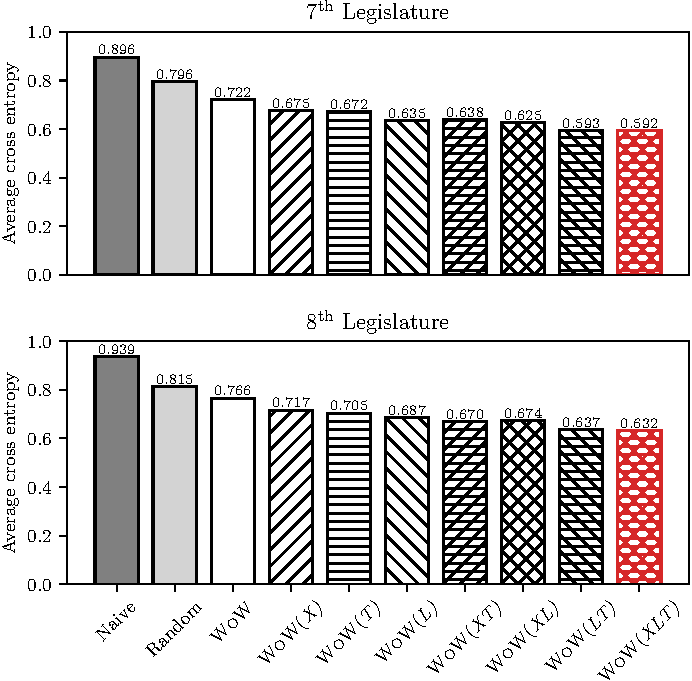
\includegraphics[width=\linewidth*3/4]{lmp-results}
	\caption{%
		Average cross-entropy loss of the baselines and our models.
		Combining the explicit, latent, and text features help obtain the best performance.
	}
	\label{lmp:fig:results}
\end{figure}

% Move to a new section?
\subsection{Interpretation of Explicit Features}

% - Explore the contribution of different explicit features to the performance of the model
To understand the contribution of the explicit features to the predictive performance, we show in Figure~\ref{lmp:fig:improvement} the decrease in cross-entropy loss of \wow{MEP} (all MEP features but the rapporteur feature), \wow{Rapp.} (rapporteur feature only), \wow{Edit}, and \wow{Dossier} over \wow.
The dossier features contribute virtually nothing to the predictive performance (the difference is at the fourth decimal point).
Similarly, for EP7, the nationality, political group, and gender features of \wow{MEP} contribute very little.
For EP8, these features improve the performance, but not as much as the edit features.
This suggests that these features have limited influence on the predictions.
Nationalities and political groups have been qualitatively analyzed in the literature in the context of their influence on MEPs' voting behaviour~\cite{hix2002parliamentary,coman2009reassessing,muhlbock2012national,lefkofridi2014multilevel}.
To the best of our knowledge, there is no analysis of their effect on the amending process.
Interestingly, for EP7, combining all features into the \wow{X} model leads to a performance boost that is greater than the sum of each individual feature groups.

\begin{figure}
  \centering
  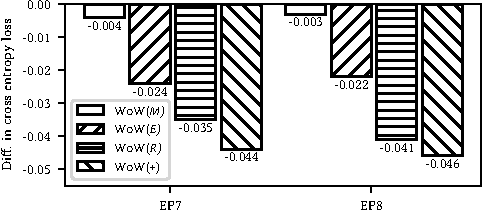
\includegraphics[width=\linewidth*3/4]{lmp-improvement}
	\caption{%
		Difference in cross-entropy loss over \wow{} of different models.
		The rapporteur feature and the edit features contribute more to the predictive performance than the MEP and dossier features.
	}
	\label{lmp:fig:improvement}
\end{figure}

\paragraph{Contribution of Explicit Features}

Let~$w_f \in \mathbf{R}$ be the value of the parameter associated with feature~$f$.
The rapporteur feature~$r$ of \wow{Rapp.} provides a greater decrease in loss.
This \textit{rapporteur advantage} complements the findings of~\citet{costello2010policy}, conducted by interviewing key informants over EP5 (1999-2004) and EP6 (2004-2009).
They show that the rapporteur, with their particular role, has some influence on the legislative process, albeit constrained.
We note that, according to our model, the rapporteur advantage has slightly increased in EP8 ($w_r=1.12$) compared to EP7 ($w_r=1.11$).

% - Interpret the values that different parameter of the explicit features take
These explicit features enable us to explain what contributes to the success of an edit.
We report here (and in subsequent sections) the results for EP8 only.
All other things being equal, a female ($w_{\text{fem}}=0.02 > -0.04 = w_{\text{mal}}$) MEP from Luxembourg and whose party belongs to the Alliance of Liberals and Democrats (center) has the highest chance to see her edit accepted.
This edit has even higher chances if it inserts ($w_{\text{ins}}=-0.02 > w_{\text{del}}=-0.11 > w_{\text{rep}}=-0.23$) a short portion of text (the feature associated with both insertion and deletion length is negative) in a part of the law that is not its body or its preamble ($w_{\text{art}}$ and~$w_{\text{rec}}$ have the lowest value among the seven article types).
Adding a justification also increases the probability of an edit being accepted ($w_{\text{jus}}=0.09$), as well as edits from the opinion committee (referred to as the "outsider committee" feature in Table~\ref{lmp:tab:features},~$w_{\text{out}} =  0.07$).

For the dossier features, our model learns that it is harder to make edits on reports, as compared to opinions (($w_{\text{rep}}=0.41 > -0.40 = w_{\text{opi}}$)).
As explained in Section~\ref{lmp:sec:dataset}, reports are voted by the whole Parliament.
Therefore, they have a greater influence on the final law, and we expect that MEPs make it more difficult for competing edits to be accepted in reports.
Surprisingly, our model also learns that it is harder to make edits for decisions (the legal acts that are binding for one member state only), as compared to regulations and directives ($w_{\text{dec}}=0.14 > 0.10 = w_{\text{reg}} = w_{\text{dir}}$).

\paragraph{Controversy of Dossiers}

Table~\ref{lmp:tab:inertia_params} provides a list of the three dossiers in EP8 with the highest inertia parameter~$d_i$ and the three dossiers with the lowest~$ d_i $.
The values of $d_i$ correlate well with the number of nodes, the number of cliques, the average size of cliques, and the edit acceptance rate.
The top-three dossiers include laws with high stakes:
The "Screening of foreign direct investments" sets a framework to better equip the EU for investments from non-EU countries.
It has crucial implications for companies, workers, governments, and citizens.
The infamous "Copyright in the Digital Single Market", considered to be a threat to freedom of expression on the Web by its opponents, sparked public protests in several cities.
The reporting committee publicized that "MEPs have rarely or never been subject to a similar degree of lobbying before"\cite{europarl2019questions}.
Finally, the "Energy efficiency labelling" updated famous labels for electrical appliances, which guide consumers in their purchases.

The number of nodes, the number of cliques, the average size of cliques, and the percentage of accepted edits correlate with the value of parameter~$ d_i$.
These four metrics are a good proxy to the level of activity by MEPs in the amending process of a given dossier.
Higher activity, possibly due to higher controversy, leads to higher value of~$d_i$.
Similarly, the skill parameters~$s_u$ enable us to quantify the influence of each MEP.
The value of~$s_u$ increases the most when MEP~$u$ wins against stronger MEPs and on dossier~$i$ with high inertia~$d_i$.
The number of edits, the proportion of successful edits, and the proportion of successful conflicts correlate with the value of parameter~$s_u$ (not shown here for space constraints).
A MEP able to propose many edits with high acceptance rate, has their political views strongly represented in laws.

% \begin{table}
%   \centering
% 	\caption{Top-3 and bottom-3 dossiers in EP8 according to their inertia parameters $d_i$.}
% 	\label{lmp:tab:inertia_params}
% 	\begin{tabular}{rllrrrr}
% 		\toprule
% 		$d_i$  & Type    & Title                                                         & \# nodes & \# cliques & avg. clique size & \% accepted \\
% 		\midrule

% 		3.304  & report  & Screening of foreign direct investments                       & 1040     & 272        & 3.1              & 2.6         \\
% 		3.204  & report  & Copyright in the Digital Single Market                        & 2657     & 577        & 4.3              & 2.6         \\
% 		3.106  & report  & Energy efficiency labelling                                   & 1292     & 319        & 3.4              & 6.0         \\

% 		\midrule

% 		-2.611 & opinion & Financial support for customs control equipment               & 60       & 1          & 2.0              & 90.0        \\
% 		-2.644 & opinion & Establishing the supervisory authorities on financial markets & 69       & 0          & 0.0              & 98.6        \\
% 		-2.849 & opinion & Unfair trading practices in the food supply chain             & 63       & 6          & 2.0              & 84.1        \\

% 		\bottomrule
% 	\end{tabular}
% \end{table}he bottom-three dossiers are all opinions, which are intrinsically less important than reports, as explained in Section~\ref{lmp:sec:background}.

% TODO: Update this table with the correct top-5 and bottom-5.
\begin{sidewaystable}
  \centering
  \caption{Inertia parameters~$d_i$ for dossiers in EP8.}
  \label{lmp:tab:inertia_params}
  \begin{tabular}{rllrrrr}
    \toprule
    $d_i$ & Type & Title & \# edits & \# conf. & avg.\ conf. size & \% accepted \\
    \midrule

    2.055 & opinion & Cost-effective emission reductions             & 1756 & 385 & 4.2 & 5.1\% \\
    1.502 & report  & Copyright in the Digital Single Market         & 2657 & 577 & 4.3 & 2.6\% \\
    1.324 & report  & Screening of foreign investments into the EU   & 1040 & 272 & 3.1 & 2.6\% \\
    1.308 & report  & Specific programme implementing Horizon Europe & 2886 & 654 & 2.7 & 13.1\% \\
    1.272 & report  & Rules of participation in Horizon Europe       & 2013 & 467 & 3.0 & 9.8\% \\

    \midrule

    -0.829 & report  & Complementing the Criminal Records Information System & 246 & 56 & 2.2 & 41.9\% \\
    -0.864 & opinion & Financial information for the detection criminals     & 81  & 2  & 2.0 & 86.4\% \\
    -0.936 & report  & Establishing a Community Code on Visas                & 259 & 61 & 2.2 & 47.5\% \\
    -0.949 & opinion & Rules of participation in Horizon Europe              & 198 & 36 & 2.2 & 58.6\% \\
    -1.445 & report  & Financial rules to the general budget of the EU       & 650 & 13 & 2.0 & 86.9\% \\

    \bottomrule
  \end{tabular}
\end{sidewaystable}

\subsection{Interpretation of Text Features}
\label{lmp:sec:intertext}

In Figure~\ref{lmp:fig:results}, we observe that the text features contribute significantly to improving the performance.
We use the learned parameter vectors~$\boldsymbol{w}_T$ and~$\boldsymbol{w}_{T'}$ of \wow{XLT} to identify words and bigrams that have the most predictive power.
First, we rank the words and bigrams of the edit text, according to the dot product of their embeddings with~$\boldsymbol{w}_T$.
The top-$k$ terms (having a positive dot product) contribute the most towards acceptance of the edit, whereas the bottom-$k$ terms (having a negative dot product) contribute most towards rejection of the edit.
The opposite holds for the terms of the title and their dot product with~$\boldsymbol{w}_{T'}$.

We look at the top~$50$ terms for each feature and prediction outcome and find some interesting patterns among these terms, although not all of them are easy to interpret.
Note that we have more than~\numprint{10000} unique terms for the edit text and more than~\numprint{1000} unique terms for the title, hence we consider only the most predictive terms near the ends of the ranking.
% A list of the top-50 terms for each feature and prediction outcome is reported in Appendix~\ref{app:accept}.

%We first examine the words and bigrams in the inserted and deleted text are predictive of acceptance.
%We see the word \textit{consumer} here, which commonly occurs in laws on consumer rights.
%This suggests that deleting provisions of the laws that give rights or benefits to consumers might be getting accepted often (possibly under the influence of lobbies), and indeed we see many such examples in the dataset.
One of the bigrams that, when deleted, is predictive of acceptance is \textit{any other}, which is commonly used to widen the scope of the law (as in ``contractual or any other duty'').
The word \textit{should}, which is used to add recommendations, is predictive of acceptance when inserted.
Adding \textit{must} and \textit{binding}, which are used for obligations, are predictive of rejection.
We see that \textit{best} is predictive of acceptance, which is commonly used to make a requirement stronger (as in ``best available scientific evidence'', ``best possible way'').
Adding \textit{positive} and \textit{positive impact} predicts acceptance, whereas adding \textit{negative} predicts rejection.
Adding the word \textit{inserted}, which commonly refers to inserting new articles in existing laws, is predictive of acceptance, whereas \textit{deleted} is predictive of rejection.

Considering the words in the context, we see that \textit{firearms}, \textit{resettlement} and \textit{privacy} are predictive of rejection.
This could be because the laws related to these topics are controversial, hence many edits are rejected due to conflicts.
For the words in the title, we see that \textit{customs}, \textit{community}, \textit{medicines}, and \textit{general budget} are predictive of acceptance, whereas \textit{market}, \textit{framework}, \textit{structural reform}, \textit{emission},  and \textit{greenhouse gas} are predictive of rejection.
This suggests the relative ease or difficulty of editing laws related to these topics, and it correlates well with the values of the difficulty parameters~$d_i$:
The top-10 dossiers with the highest difficulty parameters contain high-controversy dossiers about the screening of foreign investments, the regulation of the financial market, vast public investment programs (InvestEU), and  carbon-emission reduction and low-carbon investments,
The bottom-10 dossiers with the lowest difficulty parameters contain low-controversy dossiers about frequency bands, the attribution of the general budget to border protection and cohesion within the EU, accessibility requirements, and the information systems of criminal records.

\subsection{Interpretation of Latent Features}
% - Interpretation of the latent features
%   - In terms of ideological space for the dossier and the MEPs
%   - Explains why they improve the performance, by capturing different ideologies rather than explicit party assignment

The latent features improve the predictions overall and help capture the complex dynamics of the legislative process.
The best number of latent dimensions is~$L = 10$  for the \wow{XLT} and the \wow{LT} models, and it is~$L = 20$ for \wow{L} and \wow{XL}.
In order to interpret the latent features, we gather the latent vectors~$\bm{y}_i$ learned by \wow{XLT} into a matrix~$Y = [ \bm{y}_i ]$.
We apply principal component analysis and keep the top-10 and bottom-10 dossiers from each of the first two principal components in EP8.
We use t-SNE~\cite{maaten2008visualizing} to represent these forty dossiers in a two-dimensional space, and we show the projection in Figure~\ref{lmp:fig:tsne}.

We distinguish four clusters.
The cluster at the top contains dossiers about investment and development programmes, finance and digitalization, and sustainable development.
We interpret this cluster as \textit{investment and development}, and we highlight with blue dots the corresponding dossiers.
The cluster at the right contains dossiers about retirement, refugees, protection of consumer and workers, and limitation of financial risk.
We interpret this cluster as \textit{social security} (green triangles).
The cluster at the bottom contains dossiers about support of the defense industry and the establishment of defense funds.
It also contains dossiers about protection of workers against pollutants, international and financial protection, and rules of accession to the EU.
We interpret this cluster as \textit{defense and protection} (red crosses).
Finally, the cluster at the left contains dossiers about economic development, innovation, and businesses, as well as dossiers about unfair trading, trade secrets, and the screening of foreign investments.
We interpret this cluster as \textit{economic competitiveness} (blue dots).

\begin{figure}
  \centering
  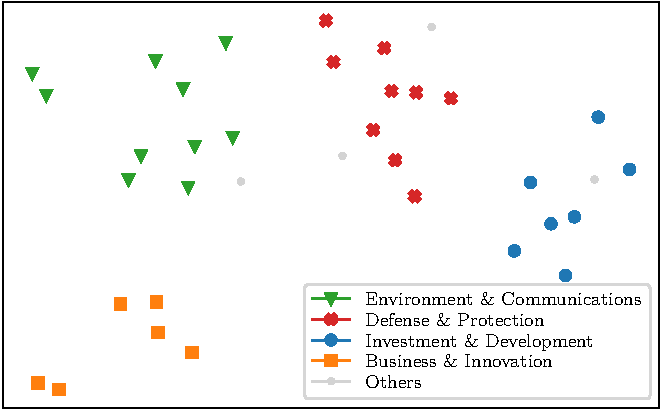
\includegraphics[width=\linewidth*3/4]{lmp-tsne}
	\caption{Visualization with t-SNE of the top-10 and bottom-10 dossiers on the first two principal components in EP8.}
	\label{lmp:fig:tsne}
\end{figure}

\subsection{Error Analysis by Conflict Size}
% - Compute the performance of high- and low-controversy dossiers
%   - Dynamics of law-making is different depending of the level of controversy
%   - We can not use the same predictor, but the hybrid models bridges the gap
% - Compute performance per committees
% - Compute performance per topic

We explore how the \wow{XLT} model performs on conflict of different sizes in the test set for EP8 (we observe a similar behaviour on EP7).
We bin the conflict size so that there are at least 100 data points in each bin.
The distribution of conflict size is exponentially decreasing:
There are 8423 conflicts of size 1 (\textit{i.e.}, an edit is in conflict with the status quo only), 3089 conflicts of size 2 (\textit{i.e.}, two edits are in conflict, as well as with the status quo),  and 107 conflicts of size 8 and more.
We compare the average cross entropy of the \wow{XLT} model with that of the random predictor and that of the \wow{} model.
In Figure~\ref{lmp:fig:error-analysis}, the loss of \wow{XLT} increases less rapidly with conflicts of larger sizes than the two baselines.
This suggests that the explicit, latent, and text features enable the model to exploit the increasing complexity of data points to make more accurate predictions.
The drop in entropy for conflicts of size 8 and more may be due to the low number of data points in this bin.

\begin{figure}
  \centering
  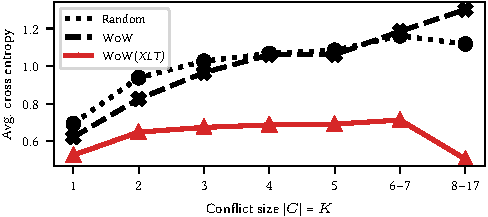
\includegraphics[width=\linewidth*3/4]{lmp-error-analysis}
	\caption{%
		Average cross-entropy loss per conflict size~$\vert \mathcal{C} \vert = K$.
		The loss of the \wow{XLT} model increases less rapidly than the loss of the baselines.
	}
	\label{lmp:fig:error-analysis}
\end{figure}

\subsection{Solving the Cold-Start Problem}
\label{lmp:sec:cold-start}

% - Predicting an edit for a new dossier
We explore how to solve the cold-start problem by defining a second predictive problem:
Given a dossier~$i$ \textit{for which we have never seen an edit}, and given a conflict~$\mathcal{C} = \{a, b, \ldots \}$, we want to predict which of the edits or the status quo wins.
We order the dossiers by the date a committee received a proposal, and we use the dossiers that contain the first 80\% of the conflicts as a training set.
We use the next 10\% as validation set, and we keep the last 10\% aside as test set.
We ensure that no edits in the training set leak into the validation and test sets.
This scenario is more realistic because we make predictions about new dossiers that the model has never observed before.

We report, in Table~\ref{lmp:tab:newdossier}, the results for \wow{Explicit}, \wow{Text}, and \wow{XT}, together with the baselines.
The latent features cannot be used for this task, as the dossier embeddings~$\vec{y}_i$ are unavailable for new dossiers.
For our models, the difficulty parameter~$d_i$ is set to the average difficulty learned in the training set.
The random predictor, which learns the prior probability of the status quo winning for each conflict size, performs the best out of all the baselines, and it outperforms \wow{Text}.
Our approach outperforms only the random predictor when including explicit features.
This suggests that the dossier features help us make more accurate predictions by learning parameter values for the type of dossier, its legal act, and its committee in charge.
In this case, adding text features further boosts the performance.

The overall performance, however, is mixed:
The improvement of \wow{XT} over the random predictor is rather small.
One possible explanation is that the legislative process might be non-stationary.
Hence, our model overfits on the training set, which is very different from the test set.
The task is also unfair to our model, as in a real setting, predictions would be made for the next dossier only.
In the current setting, we make predictions for all future dossiers.
We keep further investigations of this aspect for future work.

\begin{table}
  \centering
	\caption{Average cross entropy of the baselines and our model on predicting new, unseen dossiers.}
	\label{lmp:tab:newdossier}
	\begin{tabular}{llr}
		\toprule
		Type     & Model          & Avg.\ cross entropy \\
		\midrule
		Baseline & Naive          & 0.947               \\
		         & Random         & \textbf{0.800}      \\
		         & \wow{}       & 0.873               \\
		\midrule
		Ours     & \wow{Explicit} & 0.784               \\
		         & \wow{Text}     & 0.839               \\
		         & \wow{XT}       & \textbf{0.759}      \\
		\bottomrule
	\end{tabular}
\end{table}

%! TEX root = ../thesis.tex
\section{Related Work}
\label{sec:relwork}

%- Cite papers about text of amendments and peer-production systems
Amendment analysis in the European Parliament has been studied by the political science community on datasets of small size~\cite{kreppel1999affects,tsebelis2001legislative,kreppel2002moving,baller2017specialists}.
The effect of the rapporteur on the success of an amendment has been studied in previous legislature periods and in specific committees~\cite{finke2012proposal,hurka2013changing}.
Predicting edits on collaborative corpora of documents has been studied in the context of peer-production systems, such as Wikipedia~\cite{druck2008learning,adler2007content,sarkar2019stre} and the Linux kernel~\cite{jiang2013will,yardim2018can}.
A whole body of literature covers the conflicts between two Wikipedia edits \cite{sumi2011edit,yasseri2012dynamics} and the quantification of controversy of Wikipedia articles \cite{sepehri2012leveraging,rad2012identifying}.
The notion of conflict is, however, different in our setting, where multiple edits can be in conflict at the same time:
The task of predicting which edit will be accepted out of all the conflicting edits is more complex, and classic approaches cannot be used.
In this work, we take a peer-production viewpoint on the law-making process and propose a model of the acceptance of the legislative edits.
Our approach generalizes to any peer-production system in which (meta) features of the users and items can be extracted and in which edits can be in conflict with one another.

We use the text of the edits and dossiers as features for classification.
Text classification is a well-studied problem in natural language processing.
A simple baseline is to apply linear classifiers to term-frequency inverse document-frequency (TF-IDF) vectors~\cite{joachims1998text}.
However, these models do not capture the synonymy relation between words, hence suffer from poor generalization.
Models based on neural networks show better performance on this task~\cite{zhang2015character}.
They tend, however, to require larger datasets, and the features they learn are harder to interpret.
The fastText model~\cite{joulin2017bag} bridges the gap between the two:
It learns embeddings from linear models.
We adapt this approach to our problem of edit classification, as edits are inhomogeneous pieces of text.
Edit modelling has been studied using neural models\cite{yin2018learning,guu2018generating} that suffer from the aforementioned issues of dataset size and interpretability.
In the \warofwords{} models, we combine text features and non-text features to take into account the dynamics of the legislative process.
Legal texts also have features and structures that set them apart from other domains.
For example, the word "should" has a strong legal significance, whereas it is commonly removed as a stop word.

Our model draws inspiration from probabilistic models of choice, described in Section~\ref{in:sec:models}.
First, it borrows from the logit model to model the competitive dynamics between MEPs.
These approaches learn a real-valued score for individuals and model the probability that one individual wins over another as a function of the difference of their scores.
Second, it borrows from the Rasch model to model the competitive dynamics between MEPs and the status quo.
These approaches learn a real-valued strength for each individual and a real-valued difficulty for each item, and they model the probability that an individual wins over the item as a function of the difference of the strength and the difficulty.
Our model unifies both approaches by learning a strength for each MEP and a difficulty for each dossier, considering (i) conflicts between MEPs and (ii) conflicts between MEPs and the status quo.

%! TEX root = ../thesis.tex
\section{Summary}
\label{lmp:sec:conclusion}

In this chapter, we have introduced a new dataset of legislative edits and a model of edit outcomes.
Our dataset provides rich information on a long-term, dynamical process of interactions between parliamentarians.
Our proposed model learns a skill parameter for MEPs who propose edits and an inertia parameter for the law proposals that resist to change.
Our model also incorporates (a) explicit features of the edits, of the MEPs, and of the dossiers, (b) latent features of the MEPs and dossiers, and (c) text features of the edits and dossiers.
Each of the three classes of additional features improve the performance significantly, and the best performance is achieved by combining all features.
We interpreted the values of the learned parameters to gain insights into the legislative process.
We provided interpretation of all explicit features to characterize what makes the success of an edit more likely.
We have shown that the latent features capture the representation of MEPs and dossiers in an ideological space.
We have analyzed the words and bigrams in different parts of an edit and a dossier in terms of their influence on the acceptance probability.
We have also analyzed the performance of our model on subsets of the test set based on conflict size, and we have shown that our best model can leverage the features of the data to make more accurate predictions on conflicts of higher size than other baselines.
Finally, we have described how to use our model for predicting edits made on new, unseen dossiers.

\paragraph{Applications and Broader Impact}
We believe that approaches such as ours are helpful to political scientists, journalists and transparency observers, and to the general public:
First, it could be useful in validating theoretical hypotheses using large-scale datasets and advanced computational methods.
Second, it could help uncover lesser-known facts, such as controversial dossiers that slipped under the radar.
Finally, the greater transparency that results from these insights can enhance trust in public institutions and strengthen democratic processes.

\paragraph{Perspective}
First, we currently use pre-trained word embeddings and embeddings trained on an ad-hoc binary classification task.
We plan to explore how to learn text embeddings in an end-to-end manner using the conflictive structure of the \warofwords{} model.
Second, as shown in Section~\ref{lmp:sec:cold-start}, our model has only limited predictive power on edits made on future dossiers.
We plan to further explore how to exploit the temporality of the data and how to develop a dynamical model able to take into account the non-stationarity of the law-making process.
Finally, the current setting of the predictive task assumes that conflicts are independent of each other; because an edit can be involved in multiple conflicts, they are not always independent.
We plan to develop more advanced models by leveraging these correlations between conflicts.
For example, we plan to explore how to include latent features and text features to the mixed logit model~\citep{hensher2003mixed}.

\input{9-suppmat}

\clearpage
\bibliographystyle{ACM-Reference-Format}
\bibliography{abbreviations,war-of-words}

\end{document}
